%% LyX 2.3.7 created this file.  For more info, see http://www.lyx.org/.
%% Do not edit unless you really know what you are doing.
\documentclass[journal,article,submit,pdftex,moreauthors]{mdpi}
\usepackage[T1]{fontenc}
\usepackage[utf8]{inputenc}
\usepackage{color}
\usepackage{array}
\usepackage{float}
\usepackage{booktabs}
\usepackage{graphicx}

\makeatletter

%%%%%%%%%%%%%%%%%%%%%%%%%%%%%% LyX specific LaTeX commands.

\Title{Introducing a parallel genetic algorithm for global optimization problems}

\TitleCitation{Introducing a parallel genetic algorithm for global optimization problems}

\Author{Vasileios Charilogis$^{1}$, Ioannis G. Tsoulos$^{2,*}$}

\AuthorNames{V. Charilogis, I.G. Tsoulos}

\AuthorCitation{Charilogis V.; Tsoulos I.G.; }


\address{$^{1}$\quad{}Department of Informatics and Telecommunications,
University of Ioannina, Greece; v.charilog@uoi.gr\\
$^{2}$\quad{}Department of Informatics and Telecommunications, University
of Ioannina, Greece; itsoulos@uoi.gr}


\corres{Correspondence: itsoulos@uoi.gr;}


\firstnote{Current address: Department of Informatics and Telecommunications,
University of Ioannina, Greece.}


\secondnote{These authors contributed equally to this work.}


\abstract{The topic of efficiently finding the global minimum of multidimensional
functions finds widespread use in a multitude of problems in the modern
world. A multitude of algorithms have been proposed to solve the problems,
and Genetic Algorithms and their various variants occupy an excellent
position among them. Their popularity stems from their exceptional
performance in identifying effective solutions for optimization problems
as well as because of their adaptability to various kinds of problems.
However, Genetic Algorithms require significant computational resources
and time, prompting the need for parallel techniques. Moving in this
research direction, a new global optimization method is presented
here that exploits the use of parallel computing techniques in Genetic
Algorithms. This innovative method employs autonomous parallel computing
units, periodically sharing the optimal solutions they discover. Increasing
the number of computational threads, coupled with solution exchange
techniques, can significantly reduce the number of calls to the objective
function, thus saving computational power. Also, a stopping rule is
proposed that takes advantage of the parallel computational environment.
The proposed method was tested on a wide series of benchmark functions
from the relevant literature, and it is compared against other global
optimization techniques regarding its efficiency.}


\keyword{Parallel techniques; Global optimization; Genetic algorithms; Evolutionary
techniques}

%% Because html converters don't know tabularnewline
\providecommand{\tabularnewline}{\\}
\floatstyle{ruled}
\newfloat{algorithm}{tbp}{loa}
\providecommand{\algorithmname}{Algorithm}
\floatname{algorithm}{\protect\algorithmname}

%%%%%%%%%%%%%%%%%%%%%%%%%%%%%% User specified LaTeX commands.
%  LaTeX support: latex@mdpi.com 
%  For support, please attach all files needed for compiling as well as the log file, and specify your operating system, LaTeX version, and LaTeX editor.

%=================================================================


% For posting an early version of this manuscript as a preprint, you may use "preprints" as the journal and change "submit" to "accept". The document class line would be, e.g., \documentclass[preprints,article,accept,moreauthors,pdftex]{mdpi}. This is especially recommended for submission to arXiv, where line numbers should be removed before posting. For preprints.org, the editorial staff will make this change immediately prior to posting.

%--------------------
% Class Options:
%--------------------
%----------
% journal
%----------
% Choose between the following MDPI journals:
% acoustics, actuators, addictions, admsci, adolescents, aerospace, agriculture, agriengineering, agronomy, ai, algorithms, allergies, alloys, analytica, animals, antibiotics, antibodies, antioxidants, applbiosci, appliedchem, appliedmath, applmech, applmicrobiol, applnano, applsci, aquacj, architecture, arts, asc, asi, astronomy, atmosphere, atoms, audiolres, automation, axioms, bacteria, batteries, bdcc, behavsci, beverages, biochem, bioengineering, biologics, biology, biomass, biomechanics, biomed, biomedicines, biomedinformatics, biomimetics, biomolecules, biophysica, biosensors, biotech, birds, bloods, blsf, brainsci, breath, buildings, businesses, cancers, carbon, cardiogenetics, catalysts, cells, ceramics, challenges, chemengineering, chemistry, chemosensors, chemproc, children, chips, cimb, civileng, cleantechnol, climate, clinpract, clockssleep, cmd, coasts, coatings, colloids, colorants, commodities, compounds, computation, computers, condensedmatter, conservation, constrmater, cosmetics, covid, crops, cryptography, crystals, csmf, ctn, curroncol, currophthalmol, cyber, dairy, data, dentistry, dermato, dermatopathology, designs, diabetology, diagnostics, dietetics, digital, disabilities, diseases, diversity, dna, drones, dynamics, earth, ebj, ecologies, econometrics, economies, education, ejihpe, electricity, electrochem, electronicmat, electronics, encyclopedia, endocrines, energies, eng, engproc, ent, entomology, entropy, environments, environsciproc, epidemiologia, epigenomes, est, fermentation, fibers, fintech, fire, fishes, fluids, foods, forecasting, forensicsci, forests, foundations, fractalfract, fuels, futureinternet, futureparasites, futurepharmacol, futurephys, futuretransp, galaxies, games, gases, gastroent, gastrointestdisord, gels, genealogy, genes, geographies, geohazards, geomatics, geosciences, geotechnics, geriatrics, hazardousmatters, healthcare, hearts, hemato, heritage, highthroughput, histories, horticulturae, humanities, humans, hydrobiology, hydrogen, hydrology, hygiene, idr, ijerph, ijfs, ijgi, ijms, ijns, ijtm, ijtpp, immuno, informatics, information, infrastructures, inorganics, insects, instruments, inventions, iot, j, jal, jcdd, jcm, jcp, jcs, jdb, jeta, jfb, jfmk, jimaging, jintelligence, jlpea, jmmp, jmp, jmse, jne, jnt, jof, joitmc, jor, journalmedia, jox, jpm, jrfm, jsan, jtaer, jzbg, kidney, kidneydial, knowledge, land, languages, laws, life, liquids, literature, livers, logics, logistics, lubricants, lymphatics, machines, macromol, magnetism, magnetochemistry, make, marinedrugs, materials, materproc, mathematics, mca, measurements, medicina, medicines, medsci, membranes, merits, metabolites, metals, meteorology, methane, metrology, micro, microarrays, microbiolres, micromachines, microorganisms, microplastics, minerals, mining, modelling, molbank, molecules, mps, msf, mti, muscles, nanoenergyadv, nanomanufacturing, nanomaterials, ncrna, network, neuroglia, neurolint, neurosci, nitrogen, notspecified, nri, nursrep, nutraceuticals, nutrients, obesities, oceans, ohbm, onco, oncopathology, optics, oral, organics, organoids, osteology, oxygen, parasites, parasitologia, particles, pathogens, pathophysiology, pediatrrep, pharmaceuticals, pharmaceutics, pharmacoepidemiology, pharmacy, philosophies, photochem, photonics, phycology, physchem, physics, physiologia, plants, plasma, pollutants, polymers, polysaccharides, poultry, powders, preprints, proceedings, processes, prosthesis, proteomes, psf, psych, psychiatryint, psychoactives, publications, quantumrep, quaternary, qubs, radiation, reactions, recycling, regeneration, religions, remotesensing, reports, reprodmed, resources, rheumato, risks, robotics, ruminants, safety, sci, scipharm, seeds, sensors, separations, sexes, signals, sinusitis, skins, smartcities, sna, societies, socsci, software, soilsystems, solar, solids, sports, standards, stats, stresses, surfaces, surgeries, suschem, sustainability, symmetry, synbio, systems, taxonomy, technologies, telecom, test, textiles, thalassrep, thermo, tomography, tourismhosp, toxics, toxins, transplantology, transportation, traumacare, traumas, tropicalmed, universe, urbansci, uro, vaccines, vehicles, venereology, vetsci, vibration, viruses, vision, waste, water, wem, wevj, wind, women, world, youth, zoonoticdis 

%---------
% article
%---------
% The default type of manuscript is "article", but can be replaced by: 
% abstract, addendum, article, book, bookreview, briefreport, casereport, comment, commentary, communication, conferenceproceedings, correction, conferencereport, entry, expressionofconcern, extendedabstract, datadescriptor, editorial, essay, erratum, hypothesis, interestingimage, obituary, opinion, projectreport, reply, retraction, review, perspective, protocol, shortnote, studyprotocol, systematicreview, supfile, technicalnote, viewpoint, guidelines, registeredreport, tutorial
% supfile = supplementary materials

%----------
% submit
%----------
% The class option "submit" will be changed to "accept" by the Editorial Office when the paper is accepted. This will only make changes to the frontpage (e.g., the logo of the journal will get visible), the headings, and the copyright information. Also, line numbering will be removed. Journal info and pagination for accepted papers will also be assigned by the Editorial Office.

%------------------
% moreauthors
%------------------
% If there is only one author the class option oneauthor should be used. Otherwise use the class option moreauthors.

%---------
% pdftex
%---------
% The option pdftex is for use with pdfLaTeX. If eps figures are used, remove the option pdftex and use LaTeX and dvi2pdf.

%=================================================================
% MDPI internal commands - do not modify
\firstpage{1} 
 
\setcounter{page}{\@firstpage} 

\pubvolume{1}
\issuenum{1}
\articlenumber{0}
\pubyear{2023}
\copyrightyear{2023}
%\externaleditor{Academic Editor: Firstname Lastname} % For journal Automation, please change Academic Editor to "Communicated by"
\datereceived{}
\daterevised{ } % Comment out if no revised date
\dateaccepted{}
\datepublished{}
%\datecorrected{} % Corrected papers include a "Corrected: XXX" date in the original paper.
%\dateretracted{} % Corrected papers include a "Retracted: XXX" date in the original paper.
\hreflink{https://doi.org/} % If needed use \linebreak
%\doinum{}
%------------------------------------------------------------------
% The following line should be uncommented if the LaTeX file is uploaded to arXiv.org
%\pdfoutput=1

%=================================================================
% Add packages and commands here. The following packages are loaded in our class file: fontenc, inputenc, calc, indentfirst, fancyhdr, graphicx, epstopdf, lastpage, ifthen, lineno, float, amsmath, setspace, enumitem, mathpazo, booktabs, titlesec, etoolbox, tabto, xcolor, soul, multirow, microtype, tikz, totcount, changepage, attrib, upgreek, cleveref, amsthm, hyphenat, natbib, hyperref, footmisc, url, geometry, newfloat, caption

%=================================================================
%% Please use the following mathematics environments: Theorem, Lemma, Corollary, Proposition, Characterization, Property, Problem, Example, ExamplesandDefinitions, Hypothesis, Remark, Definition, Notation, Assumption
%% For proofs, please use the proof environment (the amsthm package is loaded by the MDPI class).

%=================================================================
% The fields PACS, MSC, and JEL may be left empty or commented out if not applicable
%\PACS{J0101}
%\MSC{}
%\JEL{}

%%%%%%%%%%%%%%%%%%%%%%%%%%%%%%%%%%%%%%%%%%
% Only for the journal Diversity
%\LSID{\url{http://}}

%%%%%%%%%%%%%%%%%%%%%%%%%%%%%%%%%%%%%%%%%%
% Only for the journal Applied Sciences:
%\featuredapplication{Authors are encouraged to provide a concise description of the specific application or a potential application of the work. This section is not mandatory.}
%%%%%%%%%%%%%%%%%%%%%%%%%%%%%%%%%%%%%%%%%%

%%%%%%%%%%%%%%%%%%%%%%%%%%%%%%%%%%%%%%%%%%
% Only for the journal Data:
%\dataset{DOI number or link to the deposited data set in cases where the data set is published or set to be published separately. If the data set is submitted and will be published as a supplement to this paper in the journal Data, this field will be filled by the editors of the journal. In this case, please make sure to submit the data set as a supplement when entering your manuscript into our manuscript editorial system.}

%\datasetlicense{license under which the data set is made available (CC0, CC-BY, CC-BY-SA, CC-BY-NC, etc.)}

%%%%%%%%%%%%%%%%%%%%%%%%%%%%%%%%%%%%%%%%%%
% Only for the journal Toxins
%\keycontribution{The breakthroughs or highlights of the manuscript. Authors can write one or two sentences to describe the most important part of the paper.}

%%%%%%%%%%%%%%%%%%%%%%%%%%%%%%%%%%%%%%%%%%
% Only for the journal Encyclopedia
%\encyclopediadef{Instead of the abstract}
%\entrylink{The Link to this entry published on the encyclopedia platform.}
%%%%%%%%%%%%%%%%%%%%%%%%%%%%%%%%%%%%%%%%%%

%%%%%%%%%%%%%%%%%%%%%%%%%%%%%%%%%%%%%%%%%%
% Only for the journal Advances in Respiratory Medicine
%\addhighlights{yes}
%\renewcommand{\addhighlights}{%

%\noindent This is an obligatory section in “Advances in Respiratory Medicine”, whose goal is to increase the discoverability and readability of the article via search engines and other scholars. Highlights should not be a copy of the abstract, but a simple text allowing the reader to quickly and simplified find out what the article is about and what can be cited from it. Each of these parts should be devoted up to 2~bullet points.\vspace{3pt}\\
%\textbf{What are the main findings?}
% \begin{itemize}[labelsep=2.5mm,topsep=-3pt]
% \item First bullet.
% \item Second bullet.
% \end{itemize}\vspace{3pt}
%\textbf{What is the implication of the main finding?}
% \begin{itemize}[labelsep=2.5mm,topsep=-3pt]
% \item First bullet.
% \item Second bullet.
% \end{itemize}
%}
%%%%%%%%%%%%%%%%%%%%%%%%%%%%%%%%%%%%%%%%%%

\@ifundefined{showcaptionsetup}{}{%
 \PassOptionsToPackage{caption=false}{subfig}}
\usepackage{subfig}
\makeatother

\begin{document}
\maketitle

\section{Introduction}

Typically the task of locating the global minimum \citep{go1} of
a function $f:S\rightarrow R,S\subset R^{n}$\textbf{ }is defined
as:
\begin{equation}
x^{*}=\mbox{arg}\min_{x\in S}f(x).\label{eq:eq1}
\end{equation}
where the set $S$ has as follows:\textbf{ 
\[
S=\left[a_{1},b_{1}\right]\otimes\left[a_{2},b_{2}\right]\otimes\ldots\left[a_{n},b_{n}\right]
\]
}The values $a_{i}$ and $b_{i}$ are the left and right bounds respectively
for the point $x_{i}$. A systematic review of the optimization procedure
can be found in the work of Fouskakis \citep{go_review}.

The previous defined problem has been tackled using a variety of methods,
which have been successfully applied to a wide range of problems in
various fields, such as Medicine \citep{go_med1,go_med2}, Chemistry
\citep{go_chem1,go_chem2}, Physics \citep{go_physics1,go_physics2,go_physics3},
Economics \citep{go_econ1,go_econ2}, etc. Global optimization methods
are divided into two main categories: deterministic and stochastic
methods \citep{go_comparison}. In the first category belong the interval
methods \citep{go_interval1,go_interval2}, where the set $S$ is
iteratively divided into subregions and those that do not contain
the global solution are discarded based on predefined criteria. Many
related works have been published in the area of deterministic methods,
such as the work of Maranas and Floudas that proposed a deterministic
method for chemical problems \citep{go_determ1},\textbf{ }the TRUST
method \citep{go_determ2},\textbf{ }the method suggested by Evtushenko
and Posypkin\citep{go_determ3} etc.\textbf{ }In the second category,
the search for the global minimum is based on randomness. Also, stochastic
optimization methods are used in most cases, since they can be programmed
more easily and they do depend on any previous information about the
objective problem. Some stochastic optimization methods that have
been used by researchers include Ant Colony Optimization \citep{go_aco1,go_aco2},
Controlled Random Search \citep{go_crs1,go_crs2,go_crs3}, Particle
Swarm Optimization \citep{go_pso1,go_pso2,go_pso3}, Simulated Annealing
\citep{go_anneal1,go_anneal2,go_anneal3}, Differential Evolution
\citep{go_de1,go_de2}, and genetic algorithms \citep{ga1,ga2,ga3}.
Finally, there is a plethora of research referring to metaheuristic
algorithms \citep{go_meta1,go_meta2,go_meta3}, offering new perspectives
and solutions to problems in various fields.

The current work proposes a series of modifications in order to effectively
parallelize the widely adopted method of Genetic Algorithms for solving
the equation \ref{eq:eq1}.\textbf{ }Genetic algorithms, initially
proposed by John Holland, constitute a fundamental technique in the
field of stochastic methods\citep{Holland}.\textbf{ }Inspired by
biology, these algorithms simulate the principles of evolution, including
genetic mutation, natural selection, and exchange of genetic material
\citep{Stender,Goldberg,Michaelewicz}. The integration of genetic
algorithms with machine learning has proven effective in addressing
complex problems and validating models. This interaction is highlighted
in applications such as the design and optimization of 5G networks,
contributing to path loss estimation and improving performance in
indoor environments \citep{Santana}. It is also applied to optimizing
the movement of digital robots \citep{Liu} and conserving energy
in industrial robots with two arms \citep{Nonoyama}. Additionally,
genetic algorithms have been employed to find optimal operating conditions
for motors \citep{Liu2}, optimize the placement of electric vehicle
charging stations \citep{Zhou}, manage energy \citep{Min}, and have
applications in other fields such as medicine \citep{Doewes,Choudhury}
and agriculture \citep{Chen}. 

Although genetic algorithms have proven to be effective, the optimization
process requires significant computational resources and time. This
emphasizes the necessity of implementing parallel techniques, as the
execution of algorithms is significantly accelerated by the combined
use of multiple computational resources. Modern parallel programming
techniques include for example the Message Passing Interface (MPI)
\citep{openmpi} or the OpenMP library \citep{opemp}. Parallel programming
techniques have also been incorporated in various cases into global
optimization, such as the combination of Simulated Annealing and parallel
techniques \citep{go_par1}, the usage of parallel methods in Particle
Swarm Optimization\citep{go_par2}, the incorporation of radial basis
functions in parallel stochastic optimization \citep{go_par3} etc.
One of the main advantages of Genetic Algorithms over other global
optimization techniques is that they can be easily parallelized and
exploit modern computing units as well as the previously mentioned
parallel programming techniques. In the relevant literature, two major
categories of parallel genetic algorithms appear: island genetic algorithms
and cellular genetic algorithms \citep{Tomohiro}. The island model
is a Parallel Genetic Algorithm (PGA), that manages several subpopulations
on separate islands, executing the genetic algorithm process on each
island simultaneously for a different set of solutions. Island models
have been utilized in various cases, such as molecular sequence alignment
\citep{ga_island0}, the quadratic assignment problem \citep{ga_island1},
placement of sensors/actuators in large structures \citep{ga_island2}
etc. Also, recently Tsoulos et al. proposed an implementation of an
island PGA \citep{pdoublepop}. In the case of the parallel cellular
model of genetic algorithms, solutions are organized into a grid.
Various diverse operators, such as crossover and mutation, are applied
to neighboring regions within the grid. For each solution, a descendant
factor is created, replacing its position within the birth region.
The model is flexible regarding the structure of the grid, neighborhood
strategies, and settings. Implementations may involve multiple processors
or graphical processing units, with information exchange possible
through physical communication networks.

The present study focuses on the island model, where the total population
is divided into independent subpopulations that operate concurrently
and independently to find candidate solutions. However, periodically,
a migration process of chromosomes with good functional values is
applied, which replaces the chromosomes that appear to contribute
to better solutions. Additionally, local optimization (LSR) is periodically
applied to expedite the overall algorithm. This approach, combined
with dissemination techniques, results in a significant improvement
in the overall performance of the genetic algorithm.

The remaining of the article follows this structure: In section \ref{sec:Method-description},
the genetic algorithm is analyzed, its parallelization is discussed,
as well as dissemination techniques (PT or migration methodologies),
and the termination criterion. Subsequently, in section \ref{sec:Experiments},
the test functions used are presented in detail, along with the experimental
results. Finally, in section \ref{sec:Conclusions}, some conclusions
are outlined, and future explorations are formulated.

\section{Method description\label{sec:Method-description}}

This section initiates with a detailed description of the base genetic
algorithm and continues providing the details of the suggested modifications.

\subsection{The Genetic Algorithm}

Genetic algorithms are inspired by natural selection and the process
of evolution in nature. In their basic form, they start with an initial
population of chromosomes, representing possible solutions to a specific
problem. Each chromosome is represented as a \textquotedbl gene\textquotedbl ,
and its length is equal to the dimension of the problem. The algorithm
processes these solutions through iterative steps, replicating and
evolving the population of solutions. In each generation, the selected
solutions are crossed and mutated to improve their fit to the problem.
As generations progress, the population converges toward solutions
with improved fit to the problem. Important factors affecting genetic
algorithm performance include population size, selection rate, crossover
and mutation probabilities, and strategic replacement of solutions.
The choice of these parameters affects the ability of the algorithm
to explore the solution space and converge to the optimal result.
Subsequently, the operation of the genetic algorithm is presented
through the replication and advancement of solution populations step
by step\citep{Yu,Lawrence}.\label{The-genetic-algorithm}:
\begin{enumerate}
\item \textbf{Initialization step}. 
\begin{enumerate}
\item \textbf{Set} $N_{c}$ as the number of chromosomes.
\item \textbf{Set} $N_{g}$ the maximum number of allowed generations. 
\item \textbf{Initialize} randomly $N_{c}$ chromosomes in $S$. Each chromosome
denotes a potential solution to the problem of Equation \ref{eq:eq1}.
\item \textbf{Set} as $p_{s}$ the selection rate of the algorithm, with
$p_{s}\le1$.
\item \textbf{Set} as $p_{m}$ the mutation rate, with $p_{m}\le1$.
\item \textbf{Set} $k$=0 as the generation counter.
\end{enumerate}
\item \textbf{Fitness calculation step. }
\begin{enumerate}
\item \textbf{For} every chromosome\textbf{ }$g_{i},\ i=1,\ldots,N_{c}$
\textbf{Calculate} the fitness $f_{i}=f\left(g_{i}\right)$ of chromosome
$g_{i}$.\textbf{\label{enu:Fitness-calculation-Step}}
\end{enumerate}
\item \textbf{Selection step}. The chromosomes are sorted with respect to
their fitness values. Denote as $N_{b}$ the integer part of $\left(1-p_{s}\right)\times N_{c}$
chromosomes with the lowest fitness values. These chromosomes will
copied to the next generation. The rest of chromosomes will be substituted
by offsprings created in the crossover procedure. Each offspring is
created from two chromosomes (parents) of the population through the
tournament selection process. The procedure of tournament selection
has as follows: A set of $N_{t}>1$ randomly selected chromosomes
is formed and the individual with the lowest fitness value from this
set is selected as parent. 
\item \textbf{Crossover step}. Two selected solutions (parents) are combined
to create new solutions (offspring). During crossover, genes are exchanged
between parents, introducing diversity. For each selected pair of
parents $(z,w)$, two additional chromosomes, represented by $\tilde{z}$
and $\tilde{w}$ , are generated through the following equations.
\begin{eqnarray}
\tilde{z_{i}} & = & a_{i}z_{i}+\left(1-a_{i}\right)w_{i}\nonumber \\
\tilde{w_{i}} & = & a_{i}w_{i}+\left(1-a_{i}\right)z_{i}\label{eq:crossover_ali-1}
\end{eqnarray}
where $i=1,\ldots,n$. The values $a_{i}$ are uniformly distributed
random numbers, with $a_{i}\in[-0.5,1.5]$ \citep{Kaelo}. 
\item \textbf{Replacement step}. 
\begin{enumerate}
\item \textbf{For} $i=N_{b}+1$ to $N_{c}$ \textbf{do}
\begin{enumerate}
\item \textbf{Replace} $g_{i}$ using the next offspring created in the
crossover procedure.
\end{enumerate}
\item \textbf{EndFor}
\end{enumerate}
\item \textbf{Mutation step}. Some genes in the offspring are randomly modified.
This introduces more diversity into the population and helps identify
new solutions.
\begin{enumerate}
\item \textbf{For} every chromosome $g_{i},\ i=1,\ldots,N_{c}$ do
\begin{enumerate}
\item \textbf{For} each element $\ j=1,\ldots,n$ of $g_{i}$ a uniformly
distributed random number $r\in\left[0,1\right]$ is drawn. The element
is altered randomly if $r\le p_{m}$.
\end{enumerate}
\item \textbf{EndFor} 
\end{enumerate}
\item \textbf{Set} $k=k+1$. If the termination criterion defined in the
work of Tsoulos \citep{Tsoulos}, which is outlined in subsection
\ref{subsec:doublebox}, is met or $k>N_{g}$ then goto Local Search
step elso goto to step \ref{enu:Fitness-calculation-Step}.
\item \textbf{Local Search step}. For improving the success in finding better
solutions, a process of local optimization search takes place. In
the present study, the Broyden Fletcher Goldfarb Shanno (BFGS) variant
proposed by Powell \citep{Powell} was employed as the local search
procedure. This procedure is applied to the chromosome in the population
with the lowest fitness value.
\end{enumerate}

\subsection{Parallelization of Genetic Algorithm and Propagation techniques}

In the parallel island model of Figure \ref{fig:Parallelization-of-genetic},
an evolving population is divided into various \textquotedbl islands\textquotedbl ,
each working concurrently to optimize a specific set of solutions.
In contrast to classical parallelization, which handles a central
population, the island model features decentralized populations evolving
independently. Each island exchanges information with others at specific
points in evolution through migration, where solutions move from one
island to another, influencing the overall convergence toward the
optimal solution. Migration settings determine how often it occurs
and which solutions are selected for exchange. Each island can follow
a similar search strategy, but for more variety or faster convergence,
different approaches can be employed. Islands may have identical or
diverse strategies, providing flexibility and efficiency in exploring
the solution space. To implement this parallel model, each island
is connected to a computational resource. For instance, as depicted
in images of Figure \ref{fig:Islands-and-propagation}, the execution
of the parallel islands model involves five islands, each managing
a distinct set of solutions using five processor units (PU). During
the migration process, information related to solutions is exchanged
among PU. In the same Figure \ref{fig:Islands-and-propagation}, the
four different techniques for spreading the chromosomes with the best
functional values are depicted. In Figure \ref{fig:Propagation-1to1},
we observe the migration of the best chromosomes from one island to
another randomly chosen. In Figure \ref{fig:Propagation-1toN}, from
a randomly chosen island to all others, in Figure \ref{fig:Propagation-Nto1},
from all islands to a randomly chosen one, and finally, in Figure
\ref{fig:Propagation-NtoN}, migration occurs from each island to
all the others.

\begin{algorithm}[H]
\begin{enumerate}
\item \textbf{Set} as $N_{I}$ the total number of parallel processing units.
\item \textbf{Set} as $N_{R}$ as the number of generations, after which
each processing unit will send its best chromosomes to the remaining
processing units.
\item \textbf{Set} $N_{P}$ as the number of migrated chromosomes between
the parallel processing units.
\item \textbf{Set} $PT$ as propagation technique.
\item \textbf{Set} $k=0$ the generation number.
\item \textbf{For} $j=1,..,N_{I}$ do in parallel\label{enu:For--do}
\begin{enumerate}
\item \textbf{Execute} an generation of the GA algorithm described in algorithm
\ref{The-genetic-algorithm} on processing unit $j$.
\item \textbf{If $K\ \mbox{mod}\ N_{R}=0,$then}
\begin{enumerate}
\item \textbf{Get} the best $N_{P}$ chromosomes from algorithm $j$.
\item \textbf{Propagate} these $N_{P}$ chromosomes to the rest of processing
units using some propagation scheme that will be described subsequently.
\end{enumerate}
\item \textbf{EndIf}
\end{enumerate}
\item \textbf{End For}
\item \textbf{Update} $k=k+1$
\item \textbf{Check} the proposed termination rule. If the termination rule
is valid, then goto step \ref{enu:Terminate-and-report} else goto
step \ref{enu:For--do}.
\begin{enumerate}
\item \textbf{Terminate} and report the best value from all processing units.
\label{enu:Terminate-and-report} Apply a local search procedure to
this located value to enhance the located global minimum.
\end{enumerate}
\end{enumerate}
\caption{The overall algorithm\label{alg:The-overall-algorithm}}
\end{algorithm}

\begin{figure}[H]
\begin{centering}
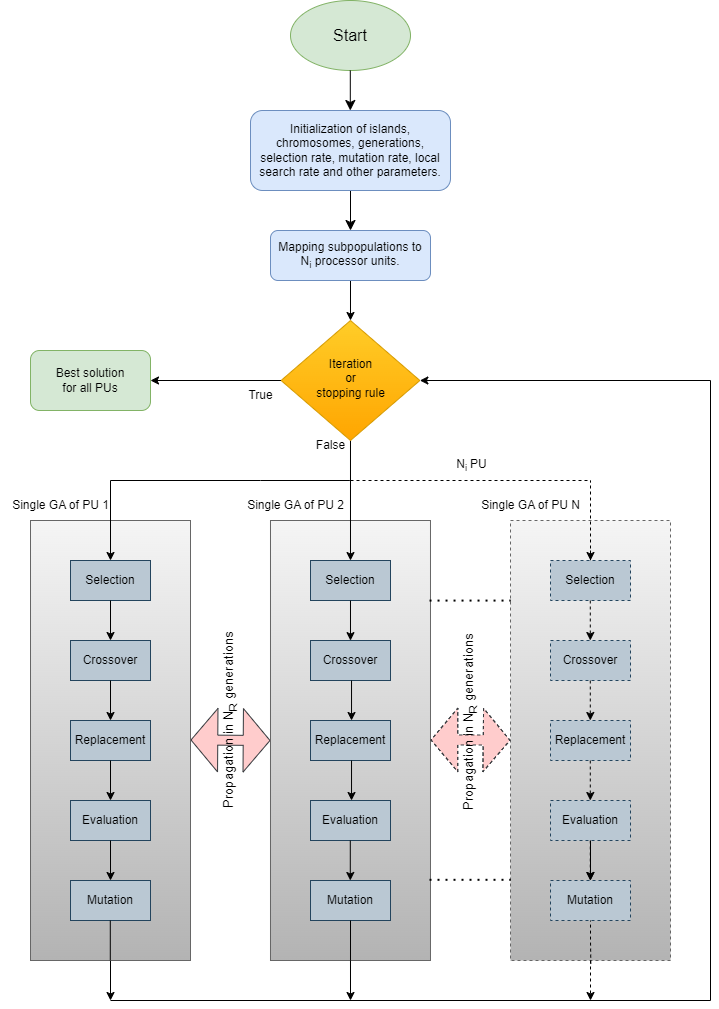
\includegraphics[scale=0.5]{pga_datagram}
\par\end{centering}
\caption{Parallelization of GA\label{fig:Parallelization-of-genetic}}
\end{figure}


\paragraph{The migration or propagation techniques, as described in this study,
are periodically and synchronously performed in $N_{R}$ iterations
on each processing unit. Below are the migration techniques that could
be defined:}
\begin{itemize}
\item 1to1: Optimal solutions migrate from a random island to another random
one, replacing the worst solutions (see figure \ref{fig:Propagation-1to1}).
\item 1toN: Optimal solutions migrate from a random island to all others,
replacing the worst solutions (see figure \ref{fig:Propagation-1toN}).
\item Nto1: All islands send their optimal solutions to a random island,
replacing the worst solutions (see figure \ref{fig:Propagation-Nto1}).
\item NtoN: All islands send their optimal solutions to all other islands,
replacing the worst solutions (see figure \ref{fig:Propagation-NtoN}).
\end{itemize}
If we assume that the migration method \textquotedbl 1toN\textquotedbl{}
is executed, then a random island will transfer chromosomes to the
other islands, except for itself. However, we kept the label \textquotedbl N\textquotedbl{}
instead of \textquotedbl N-1\textquotedbl{} because the chromosomes
exist on the island that sends them.

The number of solutions participating in the migration and replacement
process is fully customizable and will be referred to in the experiments
below.

\begin{figure}[H]
\begin{centering}
\subfloat[Propagation 1to1\label{fig:Propagation-1to1}]{\begin{centering}
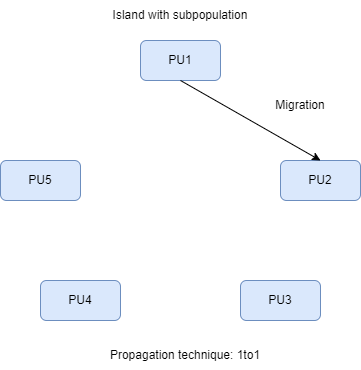
\includegraphics[scale=0.4]{parallel1}
\par\end{centering}
}\subfloat[Propagation 1toN\label{fig:Propagation-1toN}]{\begin{centering}
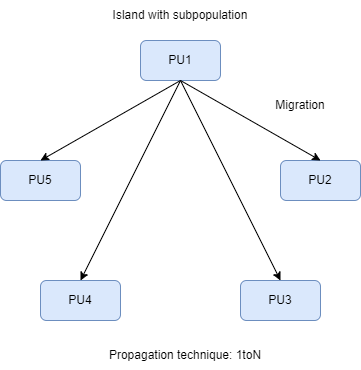
\includegraphics[scale=0.4]{parallel2}
\par\end{centering}
}
\par\end{centering}
\begin{centering}
\subfloat[Propagation Nto1\label{fig:Propagation-Nto1}]{\begin{centering}
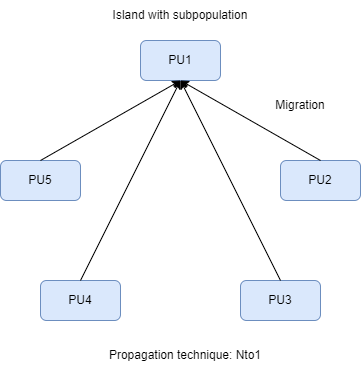
\includegraphics[scale=0.4]{parallel3}
\par\end{centering}
\centering{}}\subfloat[Propagation NtoN\label{fig:Propagation-NtoN}]{\begin{centering}
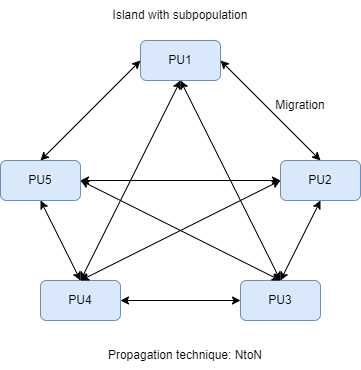
\includegraphics[scale=0.4]{parallel4}
\par\end{centering}
}
\par\end{centering}
\centering{}\caption{Islands and propagation\label{fig:Islands-and-propagation}}
\end{figure}


\subsection{Termination rule\label{subsec:doublebox}}

The termination criterion employed in this study was originally introduced
in the research conducted by Tsoulos \citep{Tsoulos} and it is formulated
as follows:
\begin{itemize}
\item In each generation $k$, the chromosome $g^{*}$ with the best functional
value $f\left(g^{*}\right)$ is retrieved from the population. If
this value does not change for a number of generations, then the algorithm
should probably terminate. 
\item Consider $\sigma^{(k)}$ as the associated variance of the quantity
$f\left(g^{*}\right)$ at generation $k$. The algorithm terminates
when:
\[
k\geq N_{g}\,\mbox{or}\,\sigma^{(k)}\leq\frac{\sigma^{\left(k_{\mbox{last}}\right)}}{2}
\]
where $k_{\mbox{last}}$ is the last generation where a lower value
for $f\left(g^{*}\right)$ was discovered.
\end{itemize}

\section{Experiments\label{sec:Experiments}}

A series of benchmark functions, found in the relevant literature
is introduced here as well as the conducted experiments and some discussion
on the experimental results. 

\subsection{Test functions}

To assess the effectiveness of the proposed method in locating the
overall minimum of functions, a set of well - known test functions,
found in the relevant literature \citep{Floudas,Montaz Ali} was employed.
The functions used here are:
\begin{itemize}
\item \textbf{Bent Cigar function}\emph{ }defined as: 
\[
f(x)=x_{1}^{2}+10^{6}\sum_{i=2}^{n}x_{i}^{2}
\]
 with the global minimum $f\left(x^{*}\right)=0$. For the conducted
experiments the value $n=10$ was used.
\item \textbf{Bf1} function (Bohachevsky 1), defined as:
\end{itemize}
\[
f(x)=x_{1}^{2}+2x_{2}^{2}-\frac{3}{10}\cos\left(3\pi x_{1}\right)-\frac{4}{10}\cos\left(4\pi x_{2}\right)+\frac{7}{10}
\]
with $x\in[-100,100]^{2}$. 
\begin{itemize}
\item \textbf{Bf2} function (Bohachevsky 2), defined as: 
\[
f(x)=x_{1}^{2}+2x_{2}^{2}-\frac{3}{10}\cos\left(3\pi x_{1}\right)\cos\left(4\pi x_{2}\right)+\frac{3}{10}
\]
with $x\in[-50,50]^{2}$. 
\item \textbf{Branin} function, given by $f(x)=\left(x_{2}-\frac{5.1}{4\pi^{2}}x_{1}^{2}+\frac{5}{\pi}x_{1}-6\right)^{2}+10\left(1-\frac{1}{8\pi}\right)\cos(x_{1})+10$
with $-5\le x_{1}\le10,\ 0\le x_{2}\le15$, with $x\in[-10,10]^{2}$. 
\item \textbf{CM} function. The Cosine Mixture function is given by 
\[
f(x)=\sum_{i=1}^{n}x_{i}^{2}-\frac{1}{10}\sum_{i=1}^{n}\cos\left(5\pi x_{i}\right)
\]
with $x\in[-1,1]^{n}$. The value $n=4$ was used in the conducted
experiments.
\item \textbf{Discus function}\emph{ }The function is defined as 
\[
f(x)=10^{6}x_{1}^{2}+\sum_{i=2}^{n}x_{i}^{2}
\]
 with global minimum $f\left(x^{*}\right)=0.$ For the conducted experiments
the value $n=10$ was used.
\item \textbf{Easom} function The function is given by the equation 
\[
f(x)=-\cos\left(x_{1}\right)\cos\left(x_{2}\right)\exp\left(\left(x_{2}-\pi\right)^{2}-\left(x_{1}-\pi\right)^{2}\right)
\]
with $x\in[-100,100]^{2}$ .
\item \textbf{Exponential} function. The function is given by 
\[
f(x)=-\exp\left(-0.5\sum_{i=1}^{n}x_{i}^{2}\right),\quad-1\le x_{i}\le1
\]
The global minimum is situated at $x^{*}=(0,0,...,0)$ with a value
$-1$. In our experiments, we applied this function for $n=4,16,64$
, and referred to the respective instances as EXP4, EXP16, EXP64,
EXP100 .
\item \textbf{Griewank2} function. The function is given by
\[
f(x)=1+\frac{1}{200}\sum_{i=1}^{2}x_{i}^{2}-\prod_{i=1}^{2}\frac{\cos(x_{i})}{\sqrt{(i)}},\quad x\in[-100,100]^{2}
\]
The global minimum is located at the $x^{*}=(0,0,...,0)$ with value
0.
\item \textbf{Gkls} function. $f(x)=\mbox{Gkls}(x,n,w)$, is a function
with $w$ local minima, described in \citep{Gaviano} with $x\in[-1,1]^{n}$
and $n$ a positive integer between 2 and 100. The value of the global
minimum is -1 and in our experiments we have used $n=2,3$ and $w=50,\ 100$. 
\item \textbf{Hansen} function. $f(x)=\sum_{i=1}^{5}i\cos\left[(i-1)x_{1}+i\right]\sum_{j=1}^{5}j\cos\left[(j+1)x_{2}+j\right]$,
$x\in[-10,10]^{2}$ . The global minimum of the function is -176.541793.
\item \textbf{Hartman 3} function. The function is given by
\[
f(x)=-\sum_{i=1}^{4}c_{i}\exp\left(-\sum_{j=1}^{3}a_{ij}\left(x_{j}-p_{ij}\right)^{2}\right)
\]
with $x\in[0,1]^{3}$ and $a=\left(\begin{array}{ccc}
3 & 10 & 30\\
0.1 & 10 & 35\\
3 & 10 & 30\\
0.1 & 10 & 35
\end{array}\right),\ c=\left(\begin{array}{c}
1\\
1.2\\
3\\
3.2
\end{array}\right)$ and
\[
p=\left(\begin{array}{ccc}
0.3689 & 0.117 & 0.2673\\
0.4699 & 0.4387 & 0.747\\
0.1091 & 0.8732 & 0.5547\\
0.03815 & 0.5743 & 0.8828
\end{array}\right)
\]
The value of global minimum is -3.862782.
\item \textbf{Hartman 6} function.
\[
f(x)=-\sum_{i=1}^{4}c_{i}\exp\left(-\sum_{j=1}^{6}a_{ij}\left(x_{j}-p_{ij}\right)^{2}\right)
\]
with $x\in[0,1]^{6}$ and $a=\left(\begin{array}{cccccc}
10 & 3 & 17 & 3.5 & 1.7 & 8\\
0.05 & 10 & 17 & 0.1 & 8 & 14\\
3 & 3.5 & 1.7 & 10 & 17 & 8\\
17 & 8 & 0.05 & 10 & 0.1 & 14
\end{array}\right),\ c=\left(\begin{array}{c}
1\\
1.2\\
3\\
3.2
\end{array}\right)$ and
\[
p=\left(\begin{array}{cccccc}
0.1312 & 0.1696 & 0.5569 & 0.0124 & 0.8283 & 0.5886\\
0.2329 & 0.4135 & 0.8307 & 0.3736 & 0.1004 & 0.9991\\
0.2348 & 0.1451 & 0.3522 & 0.2883 & 0.3047 & 0.6650\\
0.4047 & 0.8828 & 0.8732 & 0.5743 & 0.1091 & 0.0381
\end{array}\right)
\]
the value of global minimum is -3.322368.
\item \textbf{High Conditioned Elliptic} function, defined as 
\[
f(x)=\sum_{i=1}^{n}\left(10^{6}\right)^{\frac{i-1}{n-1}}x_{i}^{2}
\]
Featuring a global minimum at $f\left(x^{*}\right)=0$, the experiments
were conducted using the value $n=10$
\item \textbf{Potential} function. As a test case, the molecular conformation
corresponding to the global minimum of the energy of N atoms interacting
via the Lennard-Jones potential \citep{Lennard} is utilized. The
function to be minimized is defined as follows:
\item 
\begin{equation}
V_{LJ}(r)=4\epsilon\left[\left(\frac{\sigma}{r}\right)^{12}-\left(\frac{\sigma}{r}\right)^{6}\right]\label{eq:potential}
\end{equation}
In the current experiments two different cases were studied: $N=3,\ 5$
\item \textbf{Rastrigin} function. The function is given by 
\[
f(x)=x_{1}^{2}+x_{2}^{2}-\cos(18x_{1})-\cos(18x_{2}),\quad x\in[-1,1]^{2}
\]
\item \textbf{Shekel 7} function.
\end{itemize}
\[
f(x)=-\sum_{i=1}^{7}\frac{1}{(x-a_{i})(x-a_{i})^{T}+c_{i}}
\]

with $x\in[0,10]^{4}$ and $a=\left(\begin{array}{cccc}
4 & 4 & 4 & 4\\
1 & 1 & 1 & 1\\
8 & 8 & 8 & 8\\
6 & 6 & 6 & 6\\
3 & 7 & 3 & 7\\
2 & 9 & 2 & 9\\
5 & 3 & 5 & 3
\end{array}\right),\ c=\left(\begin{array}{c}
0.1\\
0.2\\
0.2\\
0.4\\
0.4\\
0.6\\
0.3
\end{array}\right)$. 
\begin{itemize}
\item \textbf{Shekel 5 }function.
\end{itemize}
\[
f(x)=-\sum_{i=1}^{5}\frac{1}{(x-a_{i})(x-a_{i})^{T}+c_{i}}
\]
 

with $x\in[0,10]^{4}$ and $a=\left(\begin{array}{cccc}
4 & 4 & 4 & 4\\
1 & 1 & 1 & 1\\
8 & 8 & 8 & 8\\
6 & 6 & 6 & 6\\
3 & 7 & 3 & 7
\end{array}\right),\ c=\left(\begin{array}{c}
0.1\\
0.2\\
0.2\\
0.4\\
0.4
\end{array}\right)$. 
\begin{itemize}
\item \textbf{Shekel 10} function.
\end{itemize}
\[
f(x)=-\sum_{i=1}^{10}\frac{1}{(x-a_{i})(x-a_{i})^{T}+c_{i}}
\]
 

with $x\in[0,10]^{4}$ and $a=\left(\begin{array}{cccc}
4 & 4 & 4 & 4\\
1 & 1 & 1 & 1\\
8 & 8 & 8 & 8\\
6 & 6 & 6 & 6\\
3 & 7 & 3 & 7\\
2 & 9 & 2 & 9\\
5 & 5 & 3 & 3\\
8 & 1 & 8 & 1\\
6 & 2 & 6 & 2\\
7 & 3.6 & 7 & 3.6
\end{array}\right),\ c=\left(\begin{array}{c}
0.1\\
0.2\\
0.2\\
0.4\\
0.4\\
0.6\\
0.3\\
0.7\\
0.5\\
0.6
\end{array}\right)$. 
\begin{itemize}
\item \textbf{Sinusoidal} function. The function is given by 
\[
f(x)=-\left(2.5\prod_{i=1}^{n}\sin\left(x_{i}-z\right)+\prod_{i=1}^{n}\sin\left(5\left(x_{i}-z\right)\right)\right),\quad0\le x_{i}\le\pi.
\]
The global minimum is situated at $x^{*}=(2.09435,2.09435,...,2.09435)$
with a value $f\left(x^{*}\right)=-3.5$. In the performed experiments,
we examined scenarios with $n=4,8$ and $z=\frac{\pi}{6}$. The parameter
$z$ is employed to offset the position of the global minimum \citep{Zabinsky}.
\item \textbf{Test2N} function. This function is given by the equation 
\[
f(x)=\frac{1}{2}\sum_{i=1}^{n}x_{i}^{4}-16x_{i}^{2}+5x_{i},\quad x_{i}\in[-5,5].
\]
The function has $2^{n}$ in the specified range and in our experiments
we used $n=4,5,6,7,8,9$. 
\item \textbf{Test30N} function. This function is given by 
\[
f(x)=\frac{1}{10}\sin^{2}\left(3\pi x_{1}\right)\sum_{i=2}^{n-1}\left(\left(x_{i}-1\right)^{2}\left(1+\sin^{2}\left(3\pi x_{i+1}\right)\right)\right)+\left(x_{n}-1\right)^{2}\left(1+\sin^{2}\left(2\pi x_{n}\right)\right)
\]
with $x\in[-10,10]$. The function has $30^{n}$ local minima in the
specified range and we used $n=3,4$ in the conducted experiments.
\end{itemize}

\subsection{Experimental results}

To ensure the reliability and validity of the research, experiments
were conducted 30 times and concerned the Tables \ref{tab:Comparison1}
, \ref{tab:Comparison2} and \ref{tab:Comparison4}, with parameters
consistent across all experiments as outlined in Table \ref{tab:settings1}.
In Table \ref{tab:Comparison1}, the number of objective function
invocations for each problem and its solving time for various combinations
of processing units (PU) and chromosomes are provided. In the columns
containing objective function invocation values, values in parentheses
represent the percentage of executions where the overall optimum was
successfully identified. The absence of this fraction indicates a
100\% success rate, meaning that the global minimum was found in every
run. Generally, across all problems, there is a decrease in the number
of objective function invocations and execution time as the number
of parallel computing units increases. In each case, the number of
chromosomes remains constant, i.e., 1PUx500chrom, 2PUx250chrom, etc.
This is a positive result, indicating that parallelization improves
the performance of the genetic algorithm. Figures \ref{fig:Statistical1}
and \ref{fig:Statistical2} are derived from Table \ref{tab:Comparison1}.
Statistical comparison of objective function invocations, solving
times, and execution times similarly shows performance improvement
and computation time reduction for problems as the number of computing
units increases.

Specifically, in Figure \ref{fig:Statistical1}, the objective function
invocations are halved compared to the initial invocations with only
two computational units. This reduction in invocations continues significantly
as the number of computational units increases. In Figure \ref{fig:Statistical2},
we observe a similar behavior in the algorithm termination times.
In this case, the times are significantly shorter in the parallel
process with ten (10) computational units compared to a single computational
unit. In the comparisons presented above, there is a reduction in
required computational power, as shown in Figure \ref{fig:Statistical1},
along with a decrease in the time required to find solutions, as depicted
in Figure \ref{fig:Statistical2}. In Table \ref{tab:Comparison1},
additional interesting details regarding objective function invocations
and computational times are presented, such as minimum, maximum, mean,
and standard deviation. In conclusion, as the workload is distributed
among an increasing number of computational units, there is an improvement
in performance. This reinforces the overall methodology.

In Table \ref{tab:Comparison2} the chromosome migration with the
best functional values occurs in every generation, involving a specific
number of chromosomes ten, N P =10 participating in the propagation
process. To achieve a more effective implementation of propagation
techniques, we proceeded to increase the local optimization rate applied
to Table \ref{tab:Comparison2} from 0.1\% (as presented in Table
\ref{tab:Comparison1}) to 0.5\% LSR . However, the procedure of local
optimization was maintained at certain levels because an excessive
increase would result in an elevated number of calls to the objective
function. Conversely, reducing LSR would lead to a decrease in the
success rate concerning the identification of optimal chromosomes.
In the statistical representation of Figure \ref{fig:Statistical3},
we observe the superiority of the '1 to N' propagation, meaning the
transfer of ten chromosomes from a random island to all others. Equally,
effective appears to be the 'N to N' propagation. As a general rule,
if we classify migration methods based on their performance, they
will be ranked as follows: '1toN' \ref{fig:Propagation-1toN}, 'NtoN'
\ref{fig:Propagation-NtoN}, '1to1'\ref{fig:Propagation-1to1} , and
'Nto1'\ref{fig:Propagation-Nto1} . The first two strategies, where
migration occurs across all islands, demonstrate better performance
compared to the other two, where migration only affects one island.
The success of '1toN' \ref{fig:Propagation-1toN} and 'NtoN' \ref{fig:Propagation-NtoN}
, albeit with a slight difference, appears to be due to the migration
of the best chromosomes to all islands. This leads to an improvement
in the convergence of the algorithm towards better candidate solutions
in a shorter time frame. The actual times are shown in Figure \ref{fig:Comparison3}.

For conducting experiments among stochastic methods of global optimization,
including Particle Swarm Optimization (PSO), Improved PSO (IPSO)\citep{IPSO},
Differential Evolution with random selection (DE), Differential Evolution
with tournament selection (TDE)\citep{IDE}, Genetic Algorithm (GA),
and Parallel Genetic Algorithm (PGA), certain parameters remained
constant. The population size for all methods is 500 particles or
agents or chromosomes. In PGA, the population consists of 20PUx25chrom,
while all other parameters remain the same as those described in Table
\ref{tab:Comparison1}. Any method employing LSR maintains this parameter
at the same value. The double box is a termination rule that is the
same for all methods. The values resulting from experiments in the
\ref{tab:Comparison4} table are depicted in \ref{fig:Statistical4}
and fig:\ref{fig:Comparison5} Figures. The box plots of Figure \ref{fig:Statistical4}
reveal the superiority of PGA, as objective function calls remain
at approximately 10,000 across all problems. Conversely, IPSO, DE,
and TDE (especially DE) exhibit a low number of calls in some problems,
while in others, they display significant increases. During initialization
and optimization, each method has a specific lower limit of calls,
which varies from method to method. PGA easily reaches this threshold
with very small deviations, as illustrated in the same figure. The
Figure \ref{fig:Comparison5} presents the total call values for each
method.

\begin{table}[H]
\centering{}\caption{The following settings were initially used to conduct the experiments\label{tab:settings1}}
\begin{tabular}{|c|c|c|}
\hline 
Parameter & value & Explanation\tabularnewline
\hline 
\hline 
$N_{c}$ & 500x1, 250x2, 100x5, 50x10 & Chromosomes\tabularnewline
\hline 
$N_{g}$ & 200 & Max generations\tabularnewline
\hline 
$N_{I}$ & 1, 2, 5, 10 & Processing units or islands\tabularnewline
\hline 
$N_{R}$ & no propagation in \ref{tab:Comparison1}, 1: in every generation in
\ref{tab:Comparison2} & Rate of propagation\tabularnewline
\hline 
$N_{P}$ & 0 in \ref{tab:Comparison1}, 10 : in \ref{tab:Comparison2} & Chromosomes for migration\tabularnewline
\hline 
$PT$ & no in Table \ref{tab:Comparison1}, 1to1 \ref{fig:Propagation-1to1},
1toN \ref{fig:Propagation-1toN}, Nto1 \ref{fig:Propagation-Nto1},
NtoN \ref{fig:Propagation-NtoN} & Propagation technique\tabularnewline
\hline 
$p_{s}$ & 10\% & Selection rate\tabularnewline
\hline 
$p_{m}$  & 5\% & Mutation rate\tabularnewline
\hline 
$LSR$ & 0.1\% in Table \ref{tab:Comparison1}, 0.5\% in Table \ref{tab:Comparison2} & Local search rate\tabularnewline
\hline 
\end{tabular}
\end{table}

\begin{table}[H]
\centering{}\caption{Statistical analysis comparing execution times (seconds) and function
calls across varying numbers of processor units.\label{tab:Comparison1}}
\begin{tabular}{c>{\centering}p{1cm}>{\centering}p{1cm}>{\centering}p{1cm}>{\centering}p{1cm}>{\centering}p{1cm}>{\centering}p{1cm}>{\centering}p{1cm}>{\centering}p{1cm}}
\toprule 
\textbf{\tiny{}Problems} & \textbf{\tiny{}$N_{i}=1$ $N_{c}=500$ Calls} & \textbf{\tiny{}$N_{i}=1$ $N_{c}=500$ Time} & \textbf{\tiny{}$N_{i}=2$ $N_{c}=250$ Calls} & \textbf{\tiny{}$N_{i}=2$ $N_{c}=250$ Time} & \textbf{\tiny{}$N_{i}=5$ $N_{c}=100$ Calls} & \textbf{\tiny{}$N_{i}=5$ $N_{c}=100$ Time} & \textbf{\tiny{}$N_{i}=10$ $N_{c}=50$ Calls} & \textbf{\tiny{}$N_{i}=10$ $N_{c}=50$ Time}\tabularnewline
\midrule
\midrule 
\textcolor{blue}{\tiny{}BF1} & {\tiny{}10578} & {\tiny{}0.557} & {\tiny{}10555} & {\tiny{}0.193} & {\tiny{}10533} & {\tiny{}0.126} & {\tiny{}10511} & {\tiny{}0.121}\tabularnewline
\midrule 
\textcolor{blue}{\tiny{}BF2} & {\tiny{}10568} & {\tiny{}0.554} & {\tiny{}10545} & {\tiny{}0.192} & {\tiny{}10523} & {\tiny{}0.127} & {\tiny{}10533} & {\tiny{}0.119}\tabularnewline
\midrule 
\textcolor{blue}{\tiny{}BRANIN} & {\tiny{}46793} & {\tiny{}2.308} & {\tiny{}31231} & {\tiny{}0.562} & {\tiny{}11125} & {\tiny{}0.134} & {\tiny{}10533} & {\tiny{}0.169}\tabularnewline
\midrule 
\textcolor{blue}{\tiny{}CAMEL} & {\tiny{}26537} & {\tiny{}1.338} & {\tiny{}15875} & {\tiny{}0.29} & {\tiny{}15833} & {\tiny{}0.188} & {\tiny{}10861} & {\tiny{}0.123}\tabularnewline
\midrule 
\textcolor{blue}{\tiny{}CIGAR10} & {\tiny{}10502} & {\tiny{}1.089} & {\tiny{}10577} & {\tiny{}0.383} & {\tiny{}10583} & {\tiny{}0.222} & {\tiny{}10541} & {\tiny{}0.206}\tabularnewline
\midrule 
\textcolor{blue}{\tiny{}CM4} & {\tiny{}10614} & {\tiny{}1.054} & {\tiny{}10583} & {\tiny{}0.249} & {\tiny{}10581} & {\tiny{}0.151} & {\tiny{}10556} & {\tiny{}0.139}\tabularnewline
\midrule 
\textcolor{blue}{\tiny{}DISCUS10} & {\tiny{}10548} & {\tiny{}1.09} & {\tiny{}10532} & {\tiny{}0.382} & {\tiny{}10500} & {\tiny{}0.222} & {\tiny{}10502} & {\tiny{}0.205}\tabularnewline
\midrule 
\textcolor{blue}{\tiny{}EASOM} & {\tiny{}100762} & {\tiny{}4.504} & {\tiny{}100610} & {\tiny{}1.66} & {\tiny{}94541} & {\tiny{}1.089} & {\tiny{}22845} & {\tiny{}0.248}\tabularnewline
\midrule 
\textcolor{blue}{\tiny{}ELP10} & {\tiny{}10601} & {\tiny{}1.15} & {\tiny{}10590} & {\tiny{}0.436} & {\tiny{}10574} & {\tiny{}0.26} & {\tiny{}10557} & {\tiny{}0.242}\tabularnewline
\midrule 
\textcolor{blue}{\tiny{}EXP4} & {\tiny{}16621} & {\tiny{}1.092} & {\tiny{}10587} & {\tiny{}0.249} & {\tiny{}10560} & {\tiny{}0.15} & {\tiny{}10544} & {\tiny{}0.143}\tabularnewline
\midrule 
\textcolor{blue}{\tiny{}EXP16} & {\tiny{}10680} & {\tiny{}1.336} & {\tiny{}10654} & {\tiny{}0.53} & {\tiny{}10643} & {\tiny{}0.287} & {\tiny{}10626} & {\tiny{}0.258}\tabularnewline
\midrule 
\textcolor{blue}{\tiny{}EXP64} & {\tiny{}10857} & {\tiny{}2.333} & {\tiny{}10829} & {\tiny{}1.235} & {\tiny{}10814} & {\tiny{}0.825} & {\tiny{}10830} & {\tiny{}0.728}\tabularnewline
\midrule 
\textcolor{blue}{\tiny{}EXP100} & {\tiny{}10855} & {\tiny{}3.517} & {\tiny{}10901} & {\tiny{}1.763} & {\tiny{}10868} & {\tiny{}1.25} & {\tiny{}10887} & {\tiny{}1.052}\tabularnewline
\midrule 
\textcolor{blue}{\tiny{}GKLS250} & {\tiny{}50804} & {\tiny{}2.825} & {\tiny{}25832} & {\tiny{}0.607} & {\tiny{}11711} & {\tiny{}0.194} & {\tiny{}10870(93)} & {\tiny{}0.198}\tabularnewline
\midrule 
\textcolor{blue}{\tiny{}GKLS350} & {\tiny{}40707} & {\tiny{}2.327} & {\tiny{}23720} & {\tiny{}0.522} & {\tiny{}17646} & {\tiny{}0.26} & {\tiny{}14130} & {\tiny{}0.202}\tabularnewline
\midrule 
\textcolor{blue}{\tiny{}GRIEWANK2} & {\tiny{}10555} & {\tiny{}0.565} & {\tiny{}10532} & {\tiny{}0.197} & {\tiny{}10517} & {\tiny{}0.126} & {\tiny{}10492} & {\tiny{}0.118}\tabularnewline
\midrule 
\textcolor{blue}{\tiny{}GRIEWANK10} & {\tiny{}10679} & {\tiny{}1.079} & {\tiny{}10629} & {\tiny{}0.407} & {\tiny{}10613} & {\tiny{}0.239} & {\tiny{}10609} & {\tiny{}0.22}\tabularnewline
\midrule 
\textcolor{blue}{\tiny{}POTENTIAL3} & {\tiny{}39607} & {\tiny{}2.057} & {\tiny{}34327} & {\tiny{}0.881} & {\tiny{}18313} & {\tiny{}0.34} & {\tiny{}15471} & {\tiny{}0.279}\tabularnewline
\midrule 
\textcolor{blue}{\tiny{}PONTENTIAL5} & {\tiny{}33542} & {\tiny{}1.653} & {\tiny{}33737} & {\tiny{}1.074} & {\tiny{}12040} & {\tiny{}0.34} & {\tiny{}11082} & {\tiny{}0.291}\tabularnewline
\midrule 
\textcolor{blue}{\tiny{}PONTENTIAL6} & {\tiny{}28901(3)} & {\tiny{}1.56} & {\tiny{}26419(16)} & {\tiny{}1.018} & {\tiny{}14265(3)} & {\tiny{}0.478} & {\tiny{}11109(10)} & {\tiny{}0.356}\tabularnewline
\midrule 
\textcolor{blue}{\tiny{}PONTENTIAL10} & {\tiny{}42644(13)} & {\tiny{}3.316} & {\tiny{}37897(23)} & {\tiny{}2.538} & {\tiny{}14080(10)} & {\tiny{}0.937} & {\tiny{}11319(6)} & {\tiny{}0.66}\tabularnewline
\midrule 
\textcolor{blue}{\tiny{}HANSEN} & {\tiny{}46894(90)} & {\tiny{}2.494} & {\tiny{}28191(80)} & {\tiny{}0.575} & {\tiny{}11085(56)} & {\tiny{}0.153} & {\tiny{}11065} & {\tiny{}0.158}\tabularnewline
\midrule 
\textcolor{blue}{\tiny{}HARTMAN3} & {\tiny{}22235} & {\tiny{}1.525} & {\tiny{}19030} & {\tiny{}0.379} & {\tiny{}16463} & {\tiny{}0.212} & {\tiny{}12048} & {\tiny{}0.146}\tabularnewline
\midrule 
\textcolor{blue}{\tiny{}HARTMAN6} & {\tiny{}18352} & {\tiny{}1.505} & {\tiny{}15902} & {\tiny{}0.429} & {\tiny{}16726} & {\tiny{}0.279} & {\tiny{}12243} & {\tiny{}0.196}\tabularnewline
\midrule 
\textcolor{blue}{\tiny{}RASTRIGIN} & {\tiny{}16567} & {\tiny{}0.855} & {\tiny{}10543} & {\tiny{}0.193} & {\tiny{}10521} & {\tiny{}0.125} & {\tiny{}10506} & {\tiny{}0.116}\tabularnewline
\midrule 
\textcolor{blue}{\tiny{}ROSENBROCK8} & {\tiny{}10863} & {\tiny{}0.916} & {\tiny{}10700} & {\tiny{}0.333} & {\tiny{}10698} & {\tiny{}0.199} & {\tiny{}10772} & {\tiny{}0.196}\tabularnewline
\midrule 
\textcolor{blue}{\tiny{}POSENBROCK16} & {\tiny{}10918} & {\tiny{}1.371} & {\tiny{}10946} & {\tiny{}0.516} & {\tiny{}10867} & {\tiny{}0.304} & {\tiny{}10886} & {\tiny{}0.271}\tabularnewline
\midrule 
\textcolor{blue}{\tiny{}SHEKEL5} & {\tiny{}32319(50)} & {\tiny{}2.069} & {\tiny{}17913(50)} & {\tiny{}0.412} & {\tiny{}11185(36)} & {\tiny{}0.159} & {\tiny{}11010(40)} & {\tiny{}0.15}\tabularnewline
\midrule 
\textcolor{blue}{\tiny{}SHEKEL7} & {\tiny{}51183(73)} & {\tiny{}3.277} & {\tiny{}14981(53)} & {\tiny{}0.342} & {\tiny{}11457(60)} & {\tiny{}0.163} & {\tiny{}11035(50)} & {\tiny{}0.154}\tabularnewline
\midrule 
\textcolor{blue}{\tiny{}SHEKEL10} & {\tiny{}47337(70)} & {\tiny{}2.977} & {\tiny{}46927(76)} & {\tiny{}1.113} & {\tiny{}16310(56)} & {\tiny{}0.23} & {\tiny{}11329(70)} & {\tiny{}0.152}\tabularnewline
\midrule 
\textcolor{blue}{\tiny{}SINU4} & {\tiny{}66625(83)} & {\tiny{}4.344} & {\tiny{}31511(86)} & {\tiny{}0.77} & {\tiny{}13979(73)} & {\tiny{}0.211} & {\tiny{}11004(43)} & {\tiny{}0.161}\tabularnewline
\midrule 
\textcolor{blue}{\tiny{}SINU8} & {\tiny{}29705} & {\tiny{}2.57} & {\tiny{}27613} & {\tiny{}0.987} & {\tiny{}24592} & {\tiny{}0.549} & {\tiny{}11422} & {\tiny{}0.236}\tabularnewline
\midrule 
\textcolor{blue}{\tiny{}TEST2N4} & {\tiny{}25553} & {\tiny{}1.558} & {\tiny{}17701} & {\tiny{}0.397} & {\tiny{}24763} & {\tiny{}0.359} & {\tiny{}13217} & {\tiny{}0.178}\tabularnewline
\midrule 
\textcolor{blue}{\tiny{}TEST2N5} & {\tiny{}20297} & {\tiny{}1.327} & {\tiny{}18440} & {\tiny{}0.457} & {\tiny{}16759} & {\tiny{}0.265} & {\tiny{}11483} & {\tiny{}0.168}\tabularnewline
\midrule 
\textcolor{blue}{\tiny{}TEST2N6} & {\tiny{}20450} & {\tiny{}1.311} & {\tiny{}20837} & {\tiny{}0.566} & {\tiny{}18123} & {\tiny{}0.315} & {\tiny{}11988} & {\tiny{}0.194}\tabularnewline
\midrule 
\textcolor{blue}{\tiny{}TEST2N7} & {\tiny{}26113} & {\tiny{}1.924} & {\tiny{}23940} & {\tiny{}0.723} & {\tiny{}20825} & {\tiny{}0.384} & {\tiny{}11339} & {\tiny{}0.196}\tabularnewline
\midrule 
\textcolor{blue}{\tiny{}TEST2N8} & {\tiny{}18846} & {\tiny{}1.454} & {\tiny{}18549} & {\tiny{}0.585} & {\tiny{}16700} & {\tiny{}0.329} & {\tiny{}11658} & {\tiny{}0.218}\tabularnewline
\midrule 
\textcolor{blue}{\tiny{}TEST2N9} & {\tiny{}18154} & {\tiny{}1.582} & {\tiny{}18803} & {\tiny{}0.649} & {\tiny{}17100} & {\tiny{}0.368} & {\tiny{}13299} & {\tiny{}0.262}\tabularnewline
\midrule 
\textcolor{blue}{\tiny{}TEST30N3} & {\tiny{}49235} & {\tiny{}2.46} & {\tiny{}24129} & {\tiny{}0.458} & {\tiny{}14743} & {\tiny{}0.188} & {\tiny{}12345} & {\tiny{}0.152}\tabularnewline
\midrule 
\textcolor{blue}{\tiny{}TEST30N4} & {\tiny{}29667} & {\tiny{}1.553} & {\tiny{}17501} & {\tiny{}0.358} & {\tiny{}13367} & {\tiny{}0.186} & {\tiny{}11778} & {\tiny{}0.151}\tabularnewline
\midrule 
\textbf{\textcolor{green}{\tiny{}SUM}} & \textbf{\textcolor{green}{\tiny{}1105268}} & \textbf{\textcolor{green}{\tiny{}74.376}} & \textbf{\textcolor{green}{\tiny{}851319}} & \textbf{\textcolor{green}{\tiny{}25.61}} & \textbf{\textcolor{green}{\tiny{}633126}} & \textbf{\textcolor{green}{\tiny{}12.923}} & \textbf{\textcolor{green}{\tiny{}465835}} & \textbf{\textcolor{green}{\tiny{}9.532}}\tabularnewline
\midrule 
\textbf{\textcolor{green}{\tiny{}MINIMUM}} & \textbf{\textcolor{green}{\tiny{}10502 }} & \textbf{\textcolor{green}{\tiny{}0.554 }} & \textbf{\textcolor{green}{\tiny{}10532 }} & \textbf{\textcolor{green}{\tiny{}0.192 }} & \textbf{\textcolor{green}{\tiny{}10500 }} & \textbf{\textcolor{green}{\tiny{}0.125 }} & \textbf{\textcolor{green}{\tiny{}10492 }} & \textbf{\textcolor{green}{\tiny{}0.116 }}\tabularnewline
\midrule 
\textbf{\textcolor{green}{\tiny{}MAXIMUM}} & \textbf{\textcolor{green}{\tiny{}100762 }} & \textbf{\textcolor{green}{\tiny{}4.504 }} & \textbf{\textcolor{green}{\tiny{}100610 }} & \textbf{\textcolor{green}{\tiny{}2.538 }} & \textbf{\textcolor{green}{\tiny{}94541 }} & \textbf{\textcolor{green}{\tiny{}1.25 }} & \textbf{\textcolor{green}{\tiny{}22845 }} & \textbf{\textcolor{green}{\tiny{}1.052 }}\tabularnewline
\midrule 
\textbf{\textcolor{green}{\tiny{}AVERAGE}} & \textbf{\textcolor{green}{\tiny{}27631.7 }} & \textbf{\textcolor{green}{\tiny{}1.859 }} & \textbf{\textcolor{green}{\tiny{}21282.975 }} & \textbf{\textcolor{green}{\tiny{}0.640 }} & \textbf{\textcolor{green}{\tiny{}15828.15 }} & \textbf{\textcolor{green}{\tiny{}0.323 }} & \textbf{\textcolor{green}{\tiny{}11645.875 }} & \textbf{\textcolor{green}{\tiny{}0.238 }}\tabularnewline
\midrule 
\textbf{\textcolor{green}{\tiny{}STDEV}} & \textbf{\textcolor{green}{\tiny{}19305.784 }} & \textbf{\textcolor{green}{\tiny{}0.972 }} & \textbf{\textcolor{green}{\tiny{}15829.020 }} & \textbf{\textcolor{green}{\tiny{}0.482 }} & \textbf{\textcolor{green}{\tiny{}13335.509 }} & \textbf{\textcolor{green}{\tiny{}0.260 }} & \textbf{\textcolor{green}{\tiny{}2109.230 }} & \textbf{\textcolor{green}{\tiny{}0.180 }}\tabularnewline
\bottomrule
\end{tabular}
\end{table}

\begin{figure}[H]
\centering{}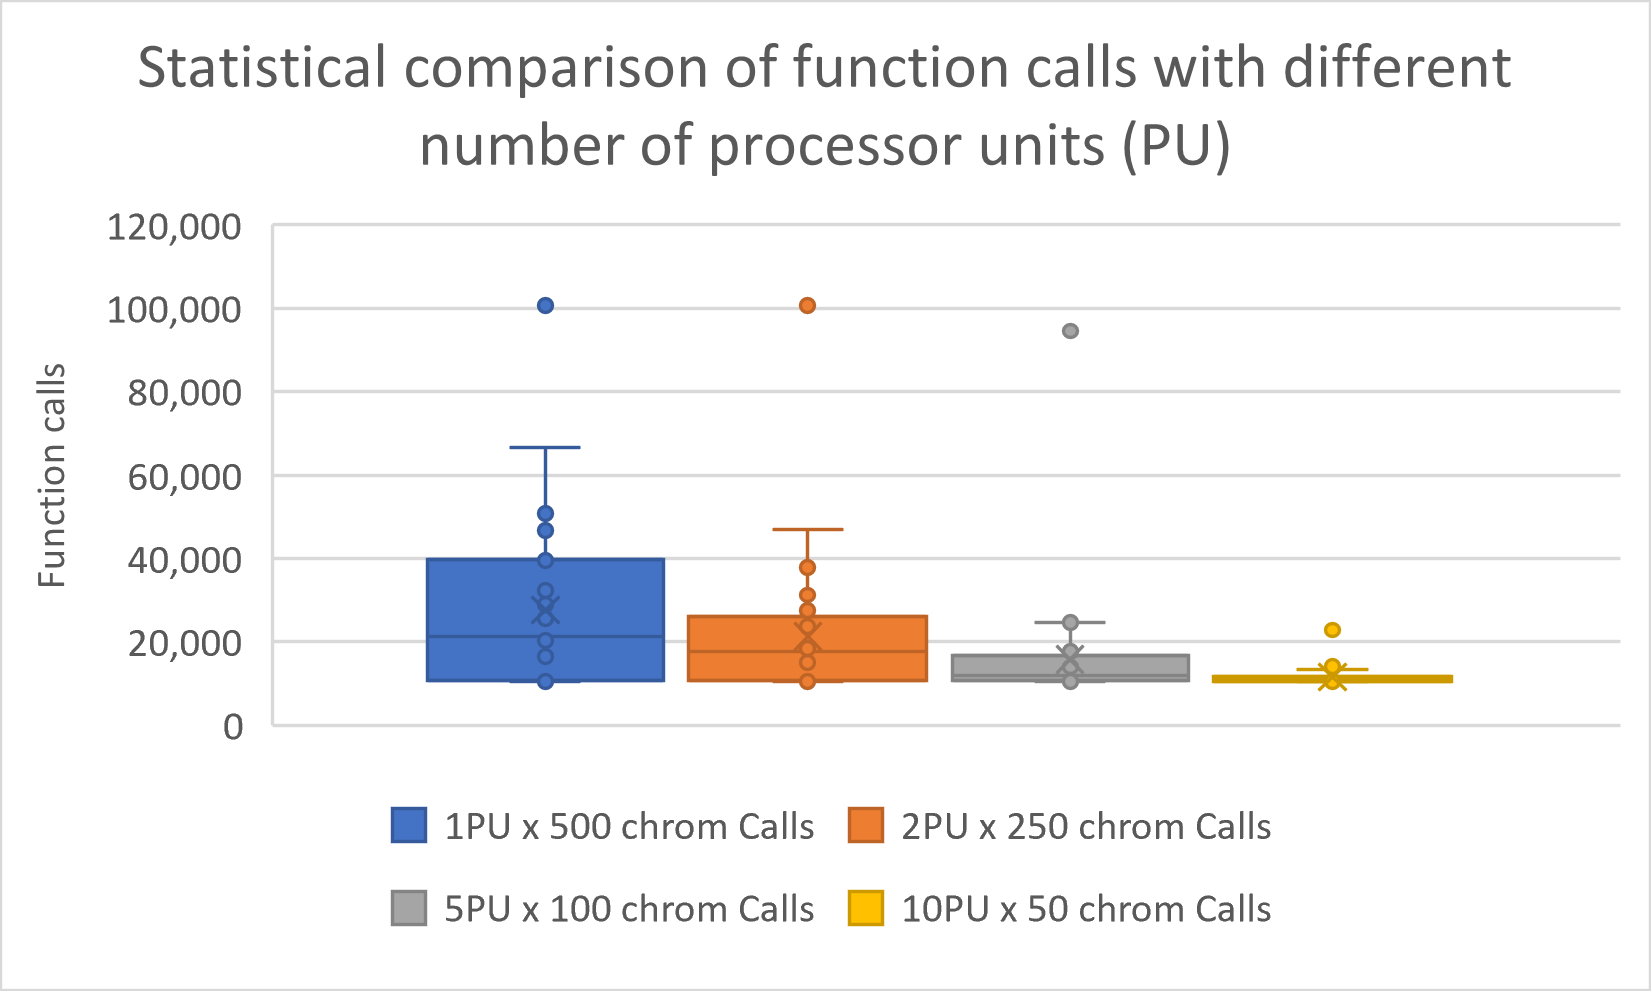
\includegraphics{7}\caption{Statistical comparison of function calls with different number of
processor units.\label{fig:Statistical1}}
\end{figure}

\begin{figure}[H]
\centering{}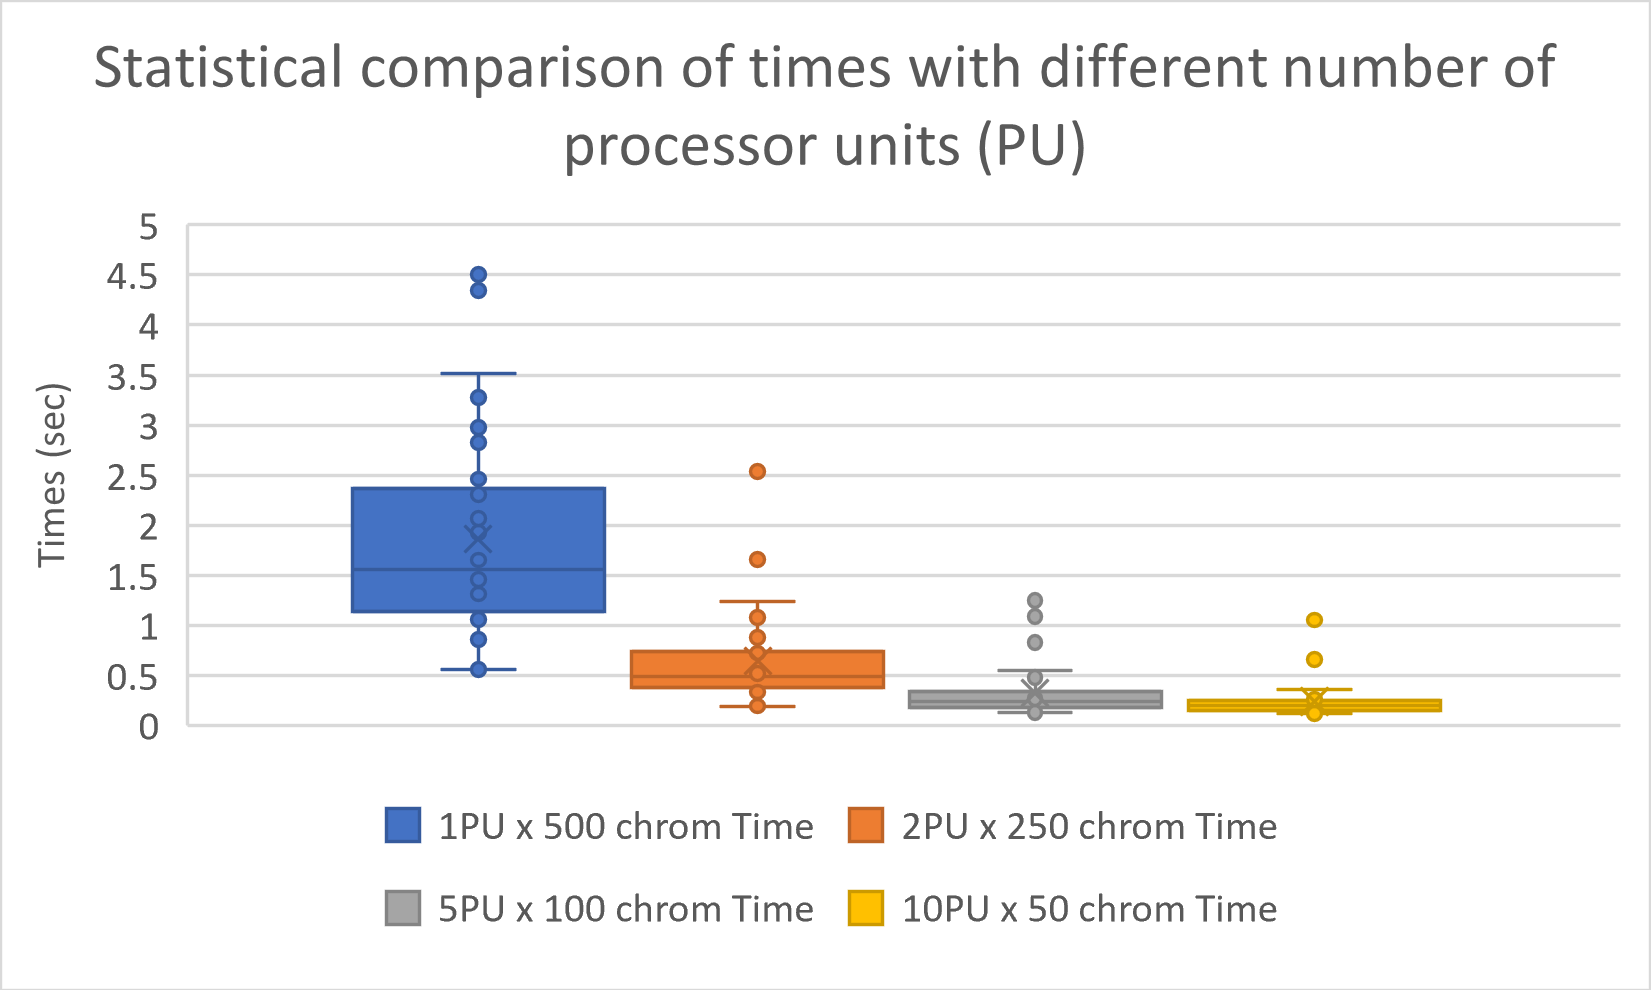
\includegraphics{8}\caption{Statistical comparison of times with different number of processor
units.\label{fig:Statistical2}}
\end{figure}

\begin{table}[H]
\begin{centering}
\caption{Evaluating function calls and time (seconds) using various propagation
techniques for comparison.\label{tab:Comparison2}}
\begin{tabular}{|c|>{\centering}p{1.1cm}|>{\centering}p{1.1cm}|>{\centering}p{0.8cm}|>{\centering}p{0.6cm}|>{\centering}p{0.8cm}|>{\centering}p{0.6cm}|>{\centering}p{0.8cm}|>{\centering}p{0.6cm}|>{\centering}p{0.8cm}|>{\centering}p{0.6cm}|}
\hline 
\textbf{\tiny{}Problems} & \textbf{\tiny{}no propagation Calls} & \textbf{\tiny{}no propagation Time} & \textbf{\tiny{}1to1 }{\tiny\par}

\textbf{\tiny{}Calls} & \textbf{\tiny{}1to1 }{\tiny\par}

\textbf{\tiny{}Time} & \textbf{\tiny{}1toN Calls} & \textbf{\tiny{}1toN Time} & \textbf{\tiny{}Nto1 Calls} & \textbf{\tiny{}Nto1 Time} & \textbf{\tiny{}NtoN Calls} & \textbf{\tiny{}NtoN Time}\tabularnewline
\hline 
\hline 
{\tiny{}BF1} & {\tiny{}10809} & {\tiny{}0.123} & {\tiny{}10741} & {\tiny{}0.127} & {\tiny{}10770} & {\tiny{}0.126} & {\tiny{}10746} & {\tiny{}0.127} & {\tiny{}10808} & {\tiny{}0.136}\tabularnewline
\hline 
{\tiny{}BF2} & {\tiny{}10725} & {\tiny{}0.124} & {\tiny{}10773} & {\tiny{}0.126} & {\tiny{}10764} & {\tiny{}0.13} & {\tiny{}10783} & {\tiny{}0.126} & {\tiny{}10731} & {\tiny{}0.136}\tabularnewline
\hline 
{\tiny{}BRANIN} & {\tiny{}48364} & {\tiny{}0.56} & {\tiny{}31470} & {\tiny{}0.397} & {\tiny{}18776} & {\tiny{}0.251} & {\tiny{}35367} & {\tiny{}0.448} & {\tiny{}19224} & {\tiny{}0.284}\tabularnewline
\hline 
{\tiny{}CAMEL} & {\tiny{}29087} & {\tiny{}0.337} & {\tiny{}18597} & {\tiny{}0.23} & {\tiny{}14429} & {\tiny{}0.185} & {\tiny{}24977} & {\tiny{}0.313} & {\tiny{}19341} & {\tiny{}0.286}\tabularnewline
\hline 
{\tiny{}CIGAR10} & {\tiny{}10854} & {\tiny{}0.233} & {\tiny{}10880} & {\tiny{}0.216} & {\tiny{}10915} & {\tiny{}0.222} & {\tiny{}10890} & {\tiny{}0.22} & {\tiny{}10869} & {\tiny{}0.235}\tabularnewline
\hline 
{\tiny{}CM4} & {\tiny{}10911} & {\tiny{}0.147} & {\tiny{}10923} & {\tiny{}0.15} & {\tiny{}10941} & {\tiny{}0.15} & {\tiny{}10918} & {\tiny{}0.15} & {\tiny{}10915} & {\tiny{}0.163}\tabularnewline
\hline 
{\tiny{}DISCUS10} & {\tiny{}10651} & {\tiny{}0.222} & {\tiny{}10632} & {\tiny{}0.213} & {\tiny{}10651} & {\tiny{}0.217} & {\tiny{}10641} & {\tiny{}0.22} & {\tiny{}10606} & {\tiny{}0.231}\tabularnewline
\hline 
{\tiny{}EASOM} & {\tiny{}99569} & {\tiny{}1.094} & {\tiny{}100163} & {\tiny{}1.106} & {\tiny{}100160} & {\tiny{}1.121} & {\tiny{}100155} & {\tiny{}1.139} & {\tiny{}98336} & {\tiny{}1.156}\tabularnewline
\hline 
{\tiny{}ELP10} & {\tiny{}10832} & {\tiny{}0.276} & {\tiny{}10902} & {\tiny{}0.261} & {\tiny{}10829} & {\tiny{}0.266} & {\tiny{}10811} & {\tiny{}0.26} & {\tiny{}10952} & {\tiny{}0.278}\tabularnewline
\hline 
{\tiny{}EXP4} & {\tiny{}10803} & {\tiny{}0.151} & {\tiny{}12037} & {\tiny{}0.167} & {\tiny{}12695} & {\tiny{}0.183} & {\tiny{}11416} & {\tiny{}0.164} & {\tiny{}10819} & {\tiny{}0.158}\tabularnewline
\hline 
{\tiny{}EXP16} & {\tiny{}11228} & {\tiny{}0.272} & {\tiny{}11259} & {\tiny{}0.276} & {\tiny{}11262} & {\tiny{}0.285} & {\tiny{}11253} & {\tiny{}0.28} & {\tiny{}11260} & {\tiny{}0.294}\tabularnewline
\hline 
{\tiny{}EXP64} & {\tiny{}12127} & {\tiny{}0.837} & {\tiny{}12204} & {\tiny{}0.848} & {\tiny{}12184} & {\tiny{}0.85} & {\tiny{}12151} & {\tiny{}0.849} & {\tiny{}12199} & {\tiny{}0.877}\tabularnewline
\hline 
{\tiny{}EXP100} & {\tiny{}12396} & {\tiny{}1.397} & {\tiny{}12376} & {\tiny{}1.4} & {\tiny{}12372} & {\tiny{}1.36} & {\tiny{}12460} & {\tiny{}1.387} & {\tiny{}12414} & {\tiny{}1.42}\tabularnewline
\hline 
{\tiny{}GKLS250} & {\tiny{}48672} & {\tiny{}0.813} & {\tiny{}55586} & {\tiny{}0.949} & {\tiny{}31493} & {\tiny{}0.564} & {\tiny{}58638} & {\tiny{}1.007} & {\tiny{}27840} & {\tiny{}0.532}\tabularnewline
\hline 
{\tiny{}GKLS350} & {\tiny{}55231} & {\tiny{}0.815} & {\tiny{}42100} & {\tiny{}0.636} & {\tiny{}28609} & {\tiny{}0.459} & {\tiny{}46923} & {\tiny{}0.72} & {\tiny{}25341} & {\tiny{}0.428}\tabularnewline
\hline 
{\tiny{}GRIEWANK2} & {\tiny{}10682} & {\tiny{}0.127} & {\tiny{}10670} & {\tiny{}0.125} & {\tiny{}10697} & {\tiny{}0.126} & {\tiny{}10683} & {\tiny{}0.127} & {\tiny{}10684} & {\tiny{}0.134}\tabularnewline
\hline 
{\tiny{}GRIEWANK10} & {\tiny{}11144} & {\tiny{}0.239} & {\tiny{}11102} & {\tiny{}0.232} & {\tiny{}11123} & {\tiny{}0.239} & {\tiny{}11171} & {\tiny{}0.229} & {\tiny{}11153} & {\tiny{}0.254}\tabularnewline
\hline 
{\tiny{}POTENTIAL3} & {\tiny{}45748} & {\tiny{}0.832} & {\tiny{}33598} & {\tiny{}0.643} & {\tiny{}17276} & {\tiny{}0.347} & {\tiny{}32603} & {\tiny{}0.631} & {\tiny{}16870} & {\tiny{}0.358}\tabularnewline
\hline 
{\tiny{}PONTENTIAL5} & {\tiny{}41946} & {\tiny{}1.156} & {\tiny{}41112} & {\tiny{}1.179} & {\tiny{}19912} & {\tiny{}0.597} & {\tiny{}37687} & {\tiny{}1.089} & {\tiny{}19622} & {\tiny{}0.614}\tabularnewline
\hline 
{\tiny{}PONTENTIAL6} & {\tiny{}46507} & {\tiny{}1.639} & {\tiny{}40518} & {\tiny{}1.449} & {\tiny{}21941} & {\tiny{}0.817} & {\tiny{}36138} & {\tiny{}1.315} & {\tiny{}21528} & {\tiny{}0.844}\tabularnewline
\hline 
{\tiny{}PONTENTIAL10} & {\tiny{}47031} & {\tiny{}3.4} & {\tiny{}45166} & {\tiny{}3.361} & {\tiny{}40212} & {\tiny{}3.239} & {\tiny{}42057} & {\tiny{}3.183} & {\tiny{}34750} & {\tiny{}2.883}\tabularnewline
\hline 
{\tiny{}HANSEN} & {\tiny{}63130} & {\tiny{}0.85} & {\tiny{}65414} & {\tiny{}0.918} & {\tiny{}39649} & {\tiny{}0.595} & {\tiny{}67369} & {\tiny{}0.947} & {\tiny{}31149} & {\tiny{}0.507}\tabularnewline
\hline 
{\tiny{}HARTMAN3} & {\tiny{}19170} & {\tiny{}0.248} & {\tiny{}20339} & {\tiny{}0.274} & {\tiny{}16280} & {\tiny{}0.226} & {\tiny{}20001} & {\tiny{}0.265} & {\tiny{}14587} & {\tiny{}0.219}\tabularnewline
\hline 
{\tiny{}HARTMAN6} & {\tiny{}23725} & {\tiny{}0.423} & {\tiny{}16856} & {\tiny{}0.285} & {\tiny{}14141} & {\tiny{}0.233} & {\tiny{}16955} & {\tiny{}0.288} & {\tiny{}13964} & {\tiny{}0.239}\tabularnewline
\hline 
{\tiny{}RASTRIGIN} & {\tiny{}11264} & {\tiny{}0.147} & {\tiny{}11256} & {\tiny{}0.132} & {\tiny{}10652} & {\tiny{}0.126} & {\tiny{}10668} & {\tiny{}0.128} & {\tiny{}11290} & {\tiny{}0.145}\tabularnewline
\hline 
{\tiny{}ROSENBROCK8} & {\tiny{}11727} & {\tiny{}0.204} & {\tiny{}11892} & {\tiny{}0.2} & {\tiny{}11681} & {\tiny{}0.203} & {\tiny{}11708} & {\tiny{}0.199} & {\tiny{}11882} & {\tiny{}0.217}\tabularnewline
\hline 
{\tiny{}POSENBROCK16} & {\tiny{}12372} & {\tiny{}0.42} & {\tiny{}12187} & {\tiny{}0.304} & {\tiny{}12394} & {\tiny{}0.313} & {\tiny{}12438} & {\tiny{}0.324} & {\tiny{}12455} & {\tiny{}0.324}\tabularnewline
\hline 
{\tiny{}SHEKEL5} & {\tiny{}44893} & {\tiny{}0.645} & {\tiny{}54184} & {\tiny{}0.751} & {\tiny{}34937} & {\tiny{}0.491} & {\tiny{}53277} & {\tiny{}0.755} & {\tiny{}40859} & {\tiny{}0.621}\tabularnewline
\hline 
{\tiny{}SHEKEL7} & {\tiny{}45722} & {\tiny{}0.638} & {\tiny{}55109} & {\tiny{}0.778} & {\tiny{}33440} & {\tiny{}0.472} & {\tiny{}49029} & {\tiny{}0.702} & {\tiny{}46066} & {\tiny{}0.696}\tabularnewline
\hline 
{\tiny{}SHEKEL10} & {\tiny{}58361} & {\tiny{}0.854} & {\tiny{}49400} & {\tiny{}0.721} & {\tiny{}32691} & {\tiny{}0.471} & {\tiny{}52798} & {\tiny{}0.783} & {\tiny{}38305} & {\tiny{}0.608}\tabularnewline
\hline 
{\tiny{}SINU4} & {\tiny{}64584} & {\tiny{}0.972} & {\tiny{}59414} & {\tiny{}0.922} & {\tiny{}36052} & {\tiny{}0.591} & {\tiny{}62924} & {\tiny{}0.972} & {\tiny{}52937} & {\tiny{}0.857}\tabularnewline
\hline 
{\tiny{}SINU8} & {\tiny{}32572} & {\tiny{}0.793} & {\tiny{}25552} & {\tiny{}0.63} & {\tiny{}19461} & {\tiny{}0.462} & {\tiny{}28744} & {\tiny{}0.716} & {\tiny{}18173} & {\tiny{}0.445}\tabularnewline
\hline 
{\tiny{}TEST2N4} & {\tiny{}23430} & {\tiny{}0.339} & {\tiny{}20474} & {\tiny{}0.3} & {\tiny{}17001} & {\tiny{}0.261} & {\tiny{}21468} & {\tiny{}0.316} & {\tiny{}18436} & {\tiny{}0.294}\tabularnewline
\hline 
{\tiny{}TEST2N5} & {\tiny{}22662} & {\tiny{}0.358} & {\tiny{}20614} & {\tiny{}0.33} & {\tiny{}16171} & {\tiny{}0.262} & {\tiny{}19697} & {\tiny{}0.316} & {\tiny{}16421} & {\tiny{}0.282}\tabularnewline
\hline 
{\tiny{}TEST2N6} & {\tiny{}21663} & {\tiny{}0.365} & {\tiny{}18721} & {\tiny{}0.323} & {\tiny{}16600} & {\tiny{}0.289} & {\tiny{}19556} & {\tiny{}0.339} & {\tiny{}14633} & {\tiny{}0.299}\tabularnewline
\hline 
{\tiny{}TEST2N7} & {\tiny{}24401} & {\tiny{}0.456} & {\tiny{}18990} & {\tiny{}0.354} & {\tiny{}15792} & {\tiny{}0.3} & {\tiny{}20967} & {\tiny{}0.405} & {\tiny{}13995} & {\tiny{}0.28}\tabularnewline
\hline 
{\tiny{}TEST2N8} & {\tiny{}21017} & {\tiny{}0.418} & {\tiny{}18532} & {\tiny{}0.369} & {\tiny{}16644} & {\tiny{}0.339} & {\tiny{}20139} & {\tiny{}0.413} & {\tiny{}13980} & {\tiny{}0.298}\tabularnewline
\hline 
{\tiny{}TEST2N9} & {\tiny{}22684} & {\tiny{}0.488} & {\tiny{}18538} & {\tiny{}0.407} & {\tiny{}16302} & {\tiny{}0.353} & {\tiny{}18929} & {\tiny{}0.421} & {\tiny{}14620} & {\tiny{}0.344}\tabularnewline
\hline 
{\tiny{}TEST30N3} & {\tiny{}24524} & {\tiny{}0.318} & {\tiny{}22799} & {\tiny{}0.296} & {\tiny{}20436} & {\tiny{}0.297} & {\tiny{}23186} & {\tiny{}0.311} & {\tiny{}19968} & {\tiny{}0.316}\tabularnewline
\hline 
{\tiny{}TEST30N4} & {\tiny{}21090} & {\tiny{}0.28} & {\tiny{}25160} & {\tiny{}0.358} & {\tiny{}21216} & {\tiny{}0.319} & {\tiny{}19444} & {\tiny{}0.276} & {\tiny{}16711} & {\tiny{}0.267}\tabularnewline
\hline 
\textbf{\tiny{}Total} & \textbf{\tiny{}1164308} & \textbf{\tiny{}24.01} & \textbf{\tiny{}1088240} & \textbf{\tiny{}22.74} & \textbf{\tiny{}829551} & \textbf{\tiny{}18.33} & \textbf{\tiny{}1097765} & \textbf{\tiny{}22.86} & \textbf{\tiny{}836693} & \textbf{\tiny{}18.95}\tabularnewline
\hline 
\end{tabular}
\par\end{centering}
\end{table}

\begin{figure}[H]
\centering{}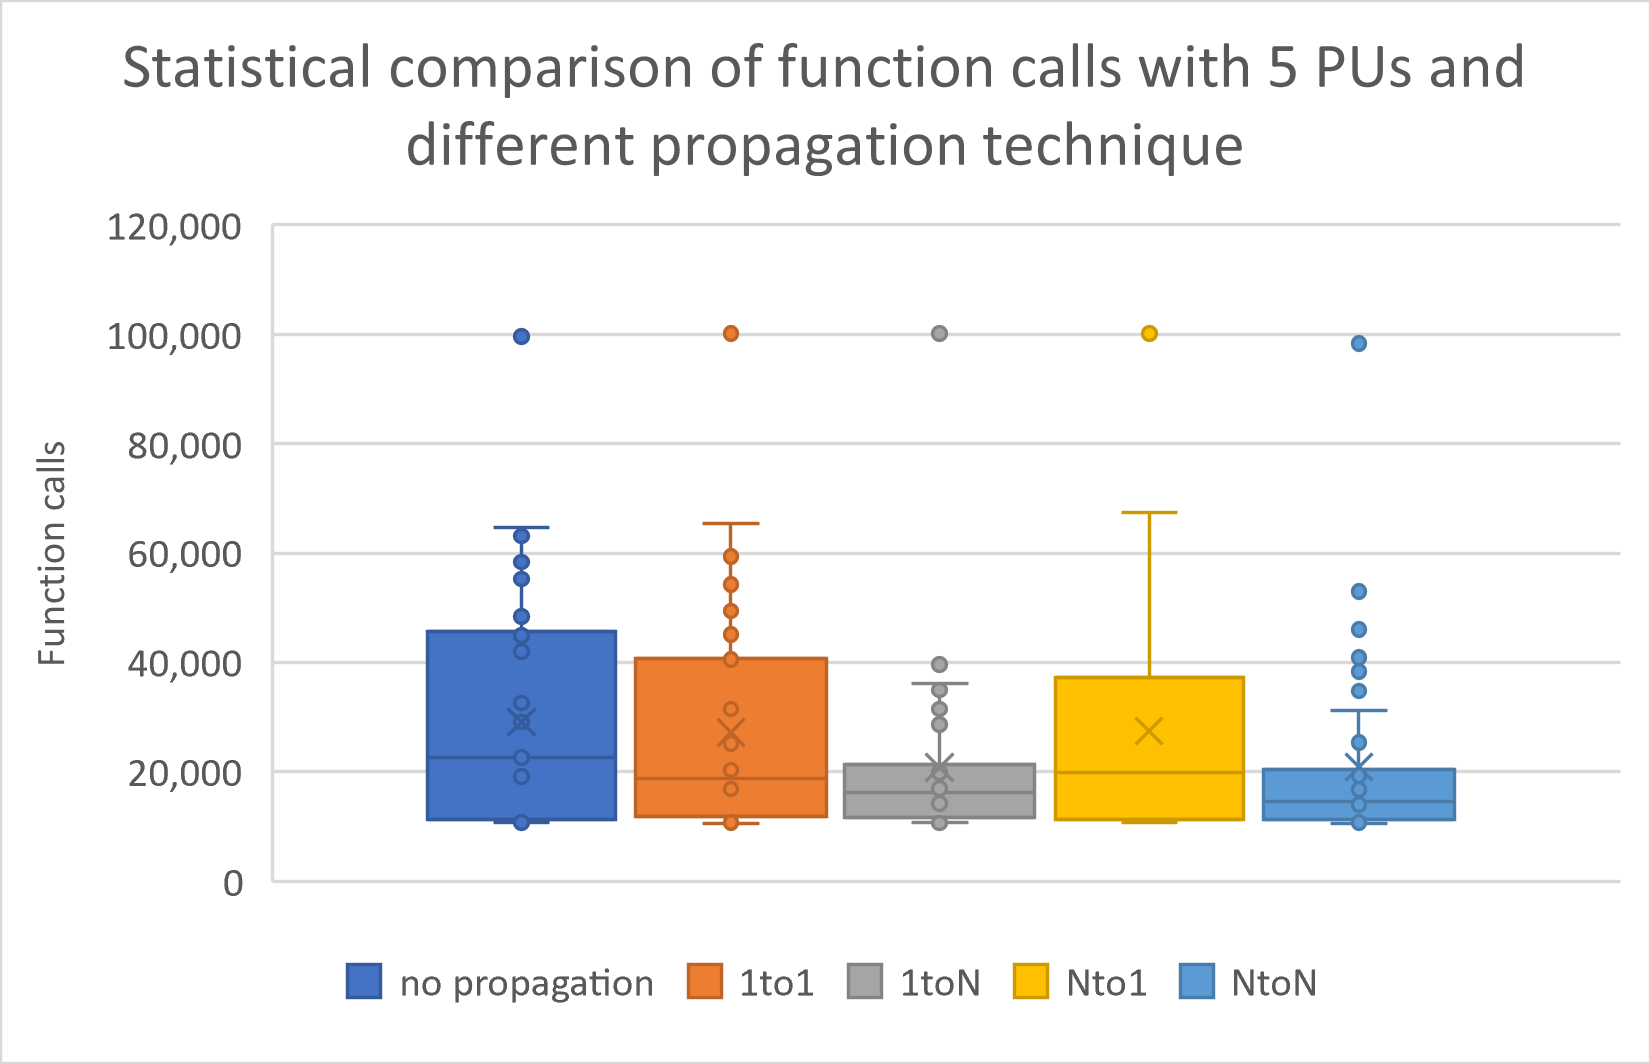
\includegraphics{4}\caption{Statistical Comparison of function calls with different number of
processor units and different propagation techniques\label{fig:Statistical3}}
\end{figure}
\begin{figure}[H]
\centering{}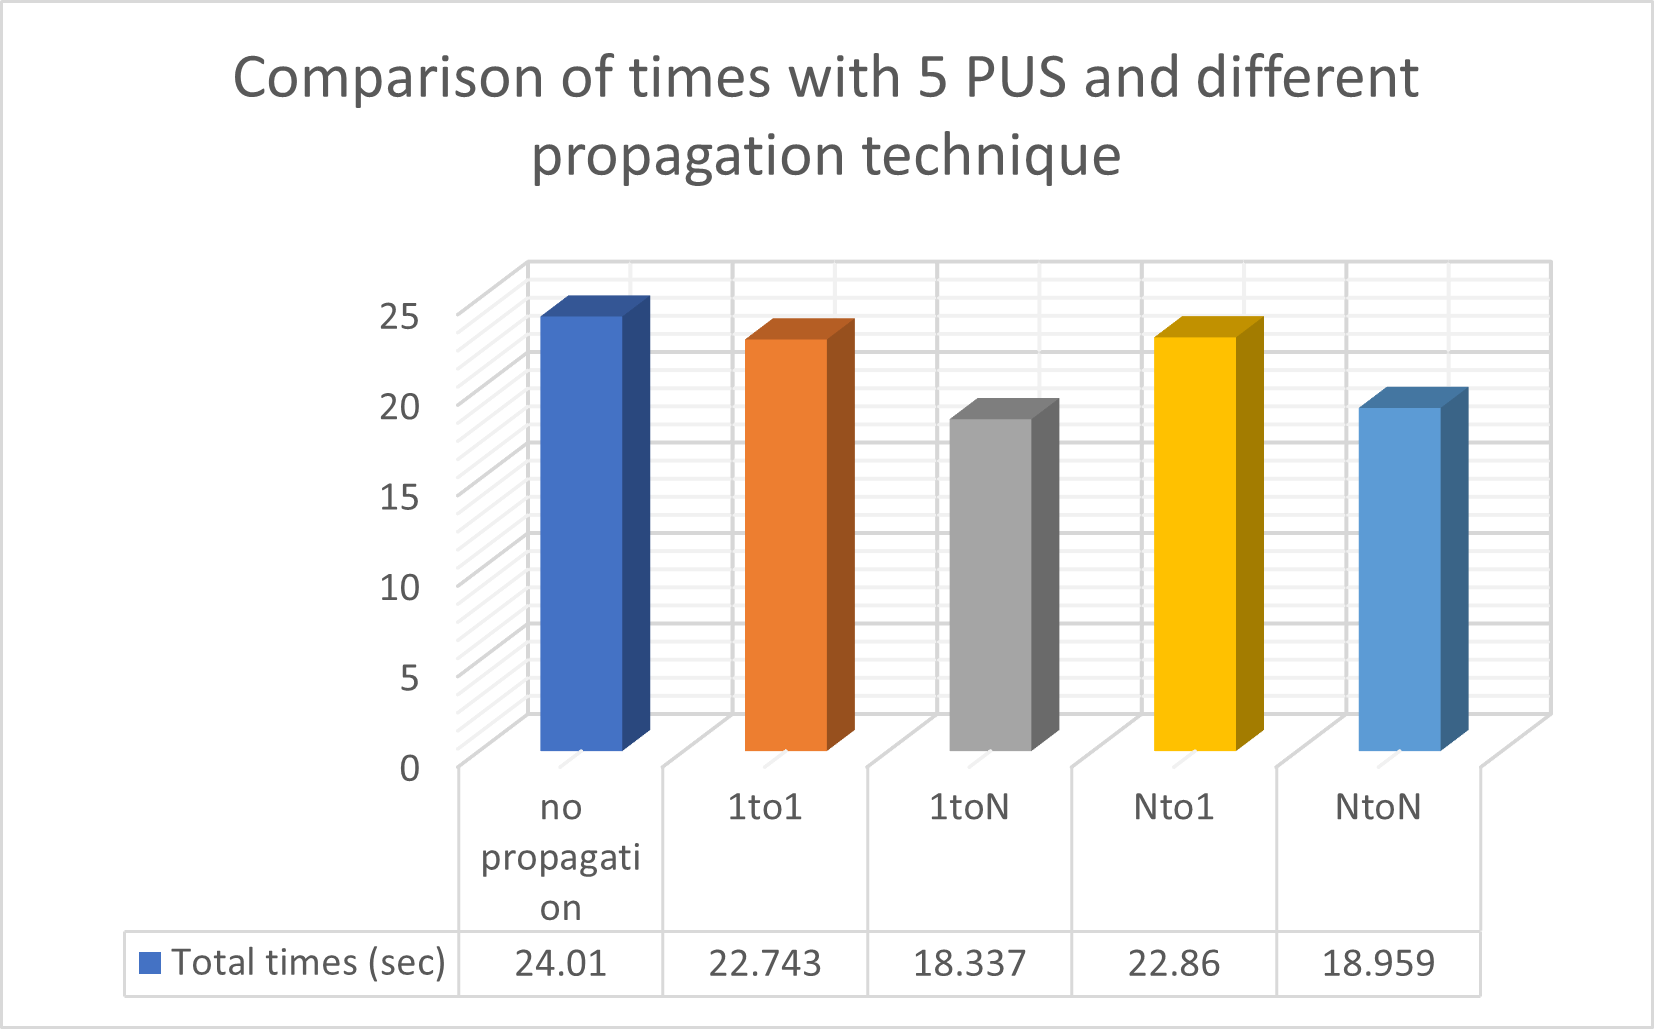
\includegraphics{6}\caption{Comparison of times (seconds) with different number of processor units
and different propagation techniques\label{fig:Comparison3}}
\end{figure}

\begin{table}[H]

\begin{centering}
\caption{Comparison of function calls using different stochastic optimization
methods\label{tab:Comparison4}}
\begin{tabular}{|c|c|c|c|c|c|c|}
\hline 
\textbf{\scriptsize{}PROBLEMS} & \textbf{\scriptsize{}PSO} & \textbf{\scriptsize{}IPSO} & \textbf{\scriptsize{}RDE} & \textbf{\scriptsize{}TDE} & \textbf{\scriptsize{}GA} & \textbf{\scriptsize{}PGA}\tabularnewline
\hline 
\hline 
{\scriptsize{}BF1} & {\scriptsize{}50398} & {\scriptsize{}11478} & {\scriptsize{}7943(86)} & {\scriptsize{}5535} & {\scriptsize{}10578} & {\scriptsize{}10501}\tabularnewline
\hline 
{\scriptsize{}BF2} & {\scriptsize{}50397} & {\scriptsize{}11292} & {\scriptsize{}8472(76)} & {\scriptsize{}5539} & {\scriptsize{}10568} & {\scriptsize{}10510}\tabularnewline
\hline 
{\scriptsize{}BRANIN} & {\scriptsize{}44800} & {\scriptsize{}10849} & {\scriptsize{}5513} & {\scriptsize{}5514} & {\scriptsize{}46793} & {\scriptsize{}10838}\tabularnewline
\hline 
{\scriptsize{}CAMEL} & {\scriptsize{}48242} & {\scriptsize{}11051} & {\scriptsize{}5555} & {\scriptsize{}5514} & {\scriptsize{}26537} & {\scriptsize{}11087}\tabularnewline
\hline 
{\scriptsize{}CIGAR10} & {\scriptsize{}50581} & {\scriptsize{}12331} & {\scriptsize{}5586} & {\scriptsize{}100573} & {\scriptsize{}10502} & {\scriptsize{}10566}\tabularnewline
\hline 
{\scriptsize{}CM4} & {\scriptsize{}48559} & {\scriptsize{}11767} & {\scriptsize{}5550} & {\scriptsize{}5538} & {\scriptsize{}10614} & {\scriptsize{}10548}\tabularnewline
\hline 
{\scriptsize{}DISCUS10} & {\scriptsize{}50523} & {\scriptsize{}14328} & {\scriptsize{}18187} & {\scriptsize{}100518} & {\scriptsize{}10548} & {\scriptsize{}10503}\tabularnewline
\hline 
{\scriptsize{}EASOM} & {\scriptsize{}21786} & {\scriptsize{}10938} & {\scriptsize{}29256} & {\scriptsize{}24691} & {\scriptsize{}100762} & {\scriptsize{}10797}\tabularnewline
\hline 
{\scriptsize{}ELP10} & {\scriptsize{}49837} & {\scriptsize{}4323} & {\scriptsize{}11933} & {\scriptsize{}100584} & {\scriptsize{}10601} & {\scriptsize{}10559}\tabularnewline
\hline 
{\scriptsize{}EXP4} & {\scriptsize{}48523} & {\scriptsize{}11041} & {\scriptsize{}46752} & {\scriptsize{}19467} & {\scriptsize{}16621} & {\scriptsize{}10503}\tabularnewline
\hline 
{\scriptsize{}EXP16} & {\scriptsize{}50518} & {\scriptsize{}10973} & {\scriptsize{}5537} & {\scriptsize{}69494} & {\scriptsize{}10680} & {\scriptsize{}10595}\tabularnewline
\hline 
{\scriptsize{}GKLS250} & {\scriptsize{}43925} & {\scriptsize{}10869} & {\scriptsize{}41016} & {\scriptsize{}11430} & {\scriptsize{}50804} & {\scriptsize{}10893(76)}\tabularnewline
\hline 
{\scriptsize{}GKLS350} & {\scriptsize{}48202} & {\scriptsize{}10750} & {\scriptsize{}56220} & {\scriptsize{}16831} & {\scriptsize{}40707} & {\scriptsize{}11555(96)}\tabularnewline
\hline 
{\scriptsize{}GRIEWANK2} & {\scriptsize{}44021} & {\scriptsize{}13514} & {\scriptsize{}5538} & {\scriptsize{}5533} & {\scriptsize{}10555} & {\scriptsize{}10498}\tabularnewline
\hline 
{\scriptsize{}GRIEWANK10} & {\scriptsize{}50557(3)} & {\scriptsize{}12258(86)} & {\scriptsize{}5612(13)} & {\scriptsize{}85742(3)} & {\scriptsize{}10679} & {\scriptsize{}10576}\tabularnewline
\hline 
{\scriptsize{}POTENTIAL3} & {\scriptsize{}49213} & {\scriptsize{}12124} & {\scriptsize{}5530} & {\scriptsize{}5523} & {\scriptsize{}39607} & {\scriptsize{}11039}\tabularnewline
\hline 
{\scriptsize{}PONTENTIAL5} & {\scriptsize{}50548} & {\scriptsize{}16027} & {\scriptsize{}5587} & {\scriptsize{}5569} & {\scriptsize{}33542} & {\scriptsize{}11134}\tabularnewline
\hline 
{\scriptsize{}PONTENTIAL6} & {\scriptsize{}50558(3)} & {\scriptsize{}24414(66)} & {\scriptsize{}5607(6)} & {\scriptsize{}5588(3)} & {\scriptsize{}28901(3)} & {\scriptsize{}11143(10)}\tabularnewline
\hline 
{\scriptsize{}PONTENTIAL10} & {\scriptsize{}50641(6)} & {\scriptsize{}31434} & {\scriptsize{}5670(3)} & {\scriptsize{}5661(6)} & {\scriptsize{}42644(13)} & {\scriptsize{}11290(20)}\tabularnewline
\hline 
{\scriptsize{}HANSEN} & {\scriptsize{}47296} & {\scriptsize{}13131} & {\scriptsize{}5522} & {\scriptsize{}5521} & {\scriptsize{}46894(90)} & {\scriptsize{}11055}\tabularnewline
\hline 
{\scriptsize{}HARTMAN3} & {\scriptsize{}47778} & {\scriptsize{}10961} & {\scriptsize{}5525} & {\scriptsize{}5522} & {\scriptsize{}22235} & {\scriptsize{}11097}\tabularnewline
\hline 
{\scriptsize{}HARTMAN6} & {\scriptsize{}50088(33)} & {\scriptsize{}11085(86)} & {\scriptsize{}5536(83)} & {\scriptsize{}5536} & {\scriptsize{}18352} & {\scriptsize{}11273}\tabularnewline
\hline 
{\scriptsize{}RASTRIGIN} & {\scriptsize{}47433} & {\scriptsize{}11594} & {\scriptsize{}5542} & {\scriptsize{}5524} & {\scriptsize{}16567} & {\scriptsize{}10506}\tabularnewline
\hline 
{\scriptsize{}ROSENBROCK8} & {\scriptsize{}50549} & {\scriptsize{}13487} & {\scriptsize{}72088} & {\scriptsize{}100503} & {\scriptsize{}10863} & {\scriptsize{}10645}\tabularnewline
\hline 
{\scriptsize{}POSENBROCK16} & {\scriptsize{}50584} & {\scriptsize{}12659} & {\scriptsize{}21517} & {\scriptsize{}10645} & {\scriptsize{}10918} & {\scriptsize{}10957}\tabularnewline
\hline 
{\scriptsize{}SHEKEL5} & {\scriptsize{}49944(33)} & {\scriptsize{}13058(93)} & {\scriptsize{}5532(86)} & {\scriptsize{}5524(93)} & {\scriptsize{}32319(50)} & {\scriptsize{}10883(43)}\tabularnewline
\hline 
{\scriptsize{}SHEKEL7} & {\scriptsize{}50062(53)} & {\scriptsize{}12134(96)} & {\scriptsize{}5533(96)} & {\scriptsize{}5523} & {\scriptsize{}51183(73)} & {\scriptsize{}10926(53)}\tabularnewline
\hline 
{\scriptsize{}SHEKEL10} & {\scriptsize{}50124(63)} & {\scriptsize{}14176} & {\scriptsize{}5535(90)} & {\scriptsize{}5523} & {\scriptsize{}47337(70)} & {\scriptsize{}11207(80)}\tabularnewline
\hline 
{\scriptsize{}SINU4} & {\scriptsize{}49239} & {\scriptsize{}11349} & {\scriptsize{}5527} & {\scriptsize{}5510} & {\scriptsize{}66625(83)} & {\scriptsize{}11063(76)}\tabularnewline
\hline 
{\scriptsize{}SINU8} & {\scriptsize{}50224} & {\scriptsize{}11295} & {\scriptsize{}5537(80)} & {\scriptsize{}5520} & {\scriptsize{}29705} & {\scriptsize{}11378}\tabularnewline
\hline 
{\scriptsize{}TEST2N4} & {\scriptsize{}50112(93)} & {\scriptsize{}13173} & {\scriptsize{}5529} & {\scriptsize{}5519} & {\scriptsize{}25553} & {\scriptsize{}11049}\tabularnewline
\hline 
{\scriptsize{}TEST2N9} & {\scriptsize{}50517(13)} & {\scriptsize{}17510(60)} & {\scriptsize{}5546(6)} & {\scriptsize{}5535(56)} & {\scriptsize{}18154} & {\scriptsize{}11145}\tabularnewline
\hline 
{\scriptsize{}TEST30N3} & {\scriptsize{}44301} & {\scriptsize{}19638} & {\scriptsize{}5515} & {\scriptsize{}5511} & {\scriptsize{}49235} & {\scriptsize{}11051}\tabularnewline
\hline 
{\scriptsize{}TEST30N4} & {\scriptsize{}49177} & {\scriptsize{}20839} & {\scriptsize{}5514} & {\scriptsize{}5511} & {\scriptsize{}29667} & {\scriptsize{}11301}\tabularnewline
\hline 
\textbf{\scriptsize{}TOTAL} & \textbf{\footnotesize{}1639257} & \textbf{\footnotesize{}457850} & \textbf{\footnotesize{}446562} & \textbf{\footnotesize{}767771} & \textbf{\footnotesize{}997850} & \textbf{\footnotesize{}370671}\tabularnewline
\hline 
\end{tabular}
\par\end{centering}
\end{table}

\begin{figure}[H]

\begin{centering}
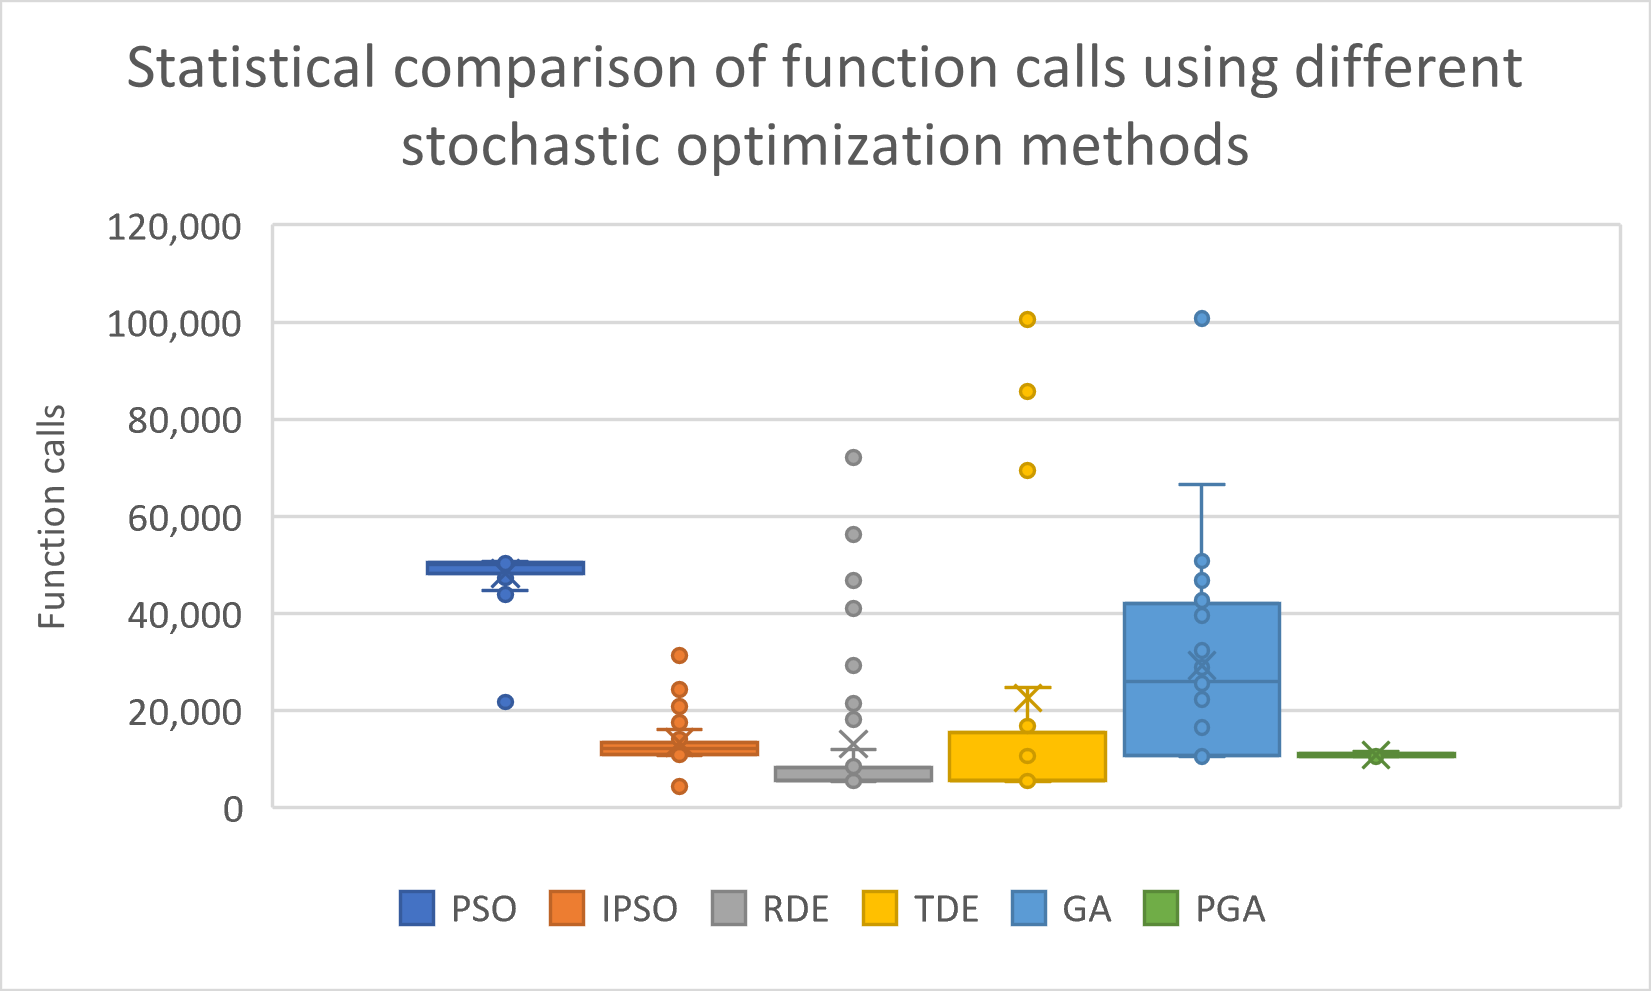
\includegraphics{9}\caption{Statistical comparison of function calls using different stochastic
optimization methods\label{fig:Statistical4}}
\par\end{centering}
\end{figure}

\begin{figure}[H]

\centering{}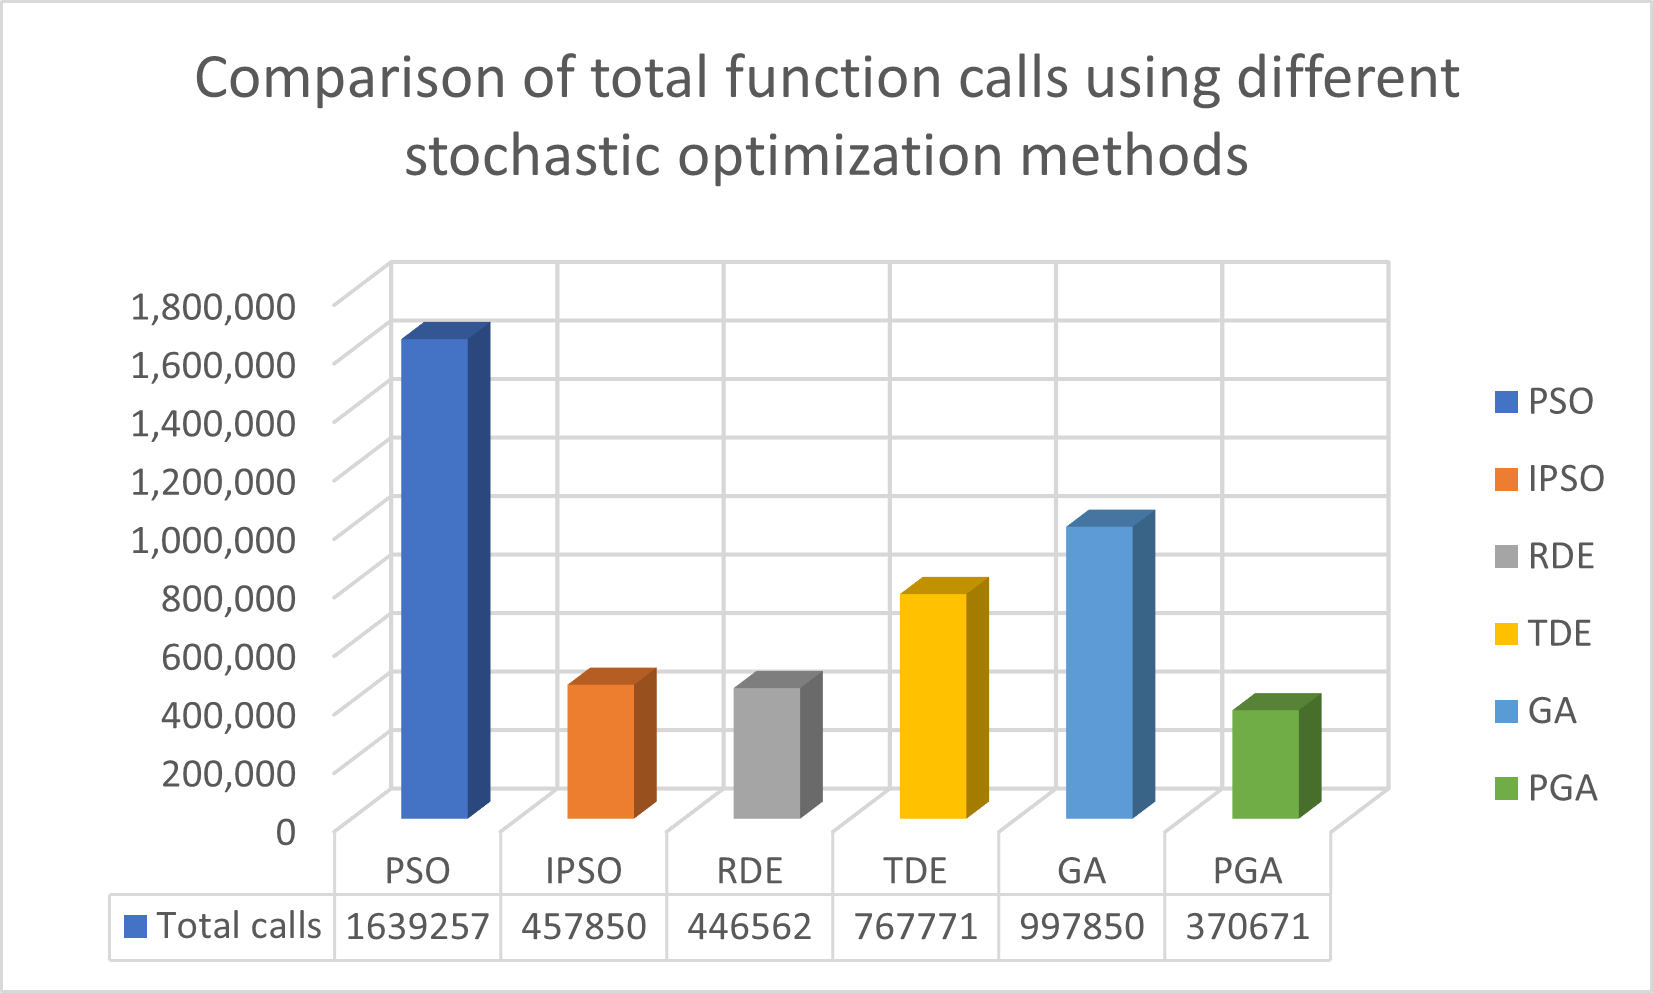
\includegraphics{10}\caption{Comparison of total function calls using different stochastic optimization
methods\label{fig:Comparison5}}
\end{figure}

\begin{figure}[H]

\begin{centering}
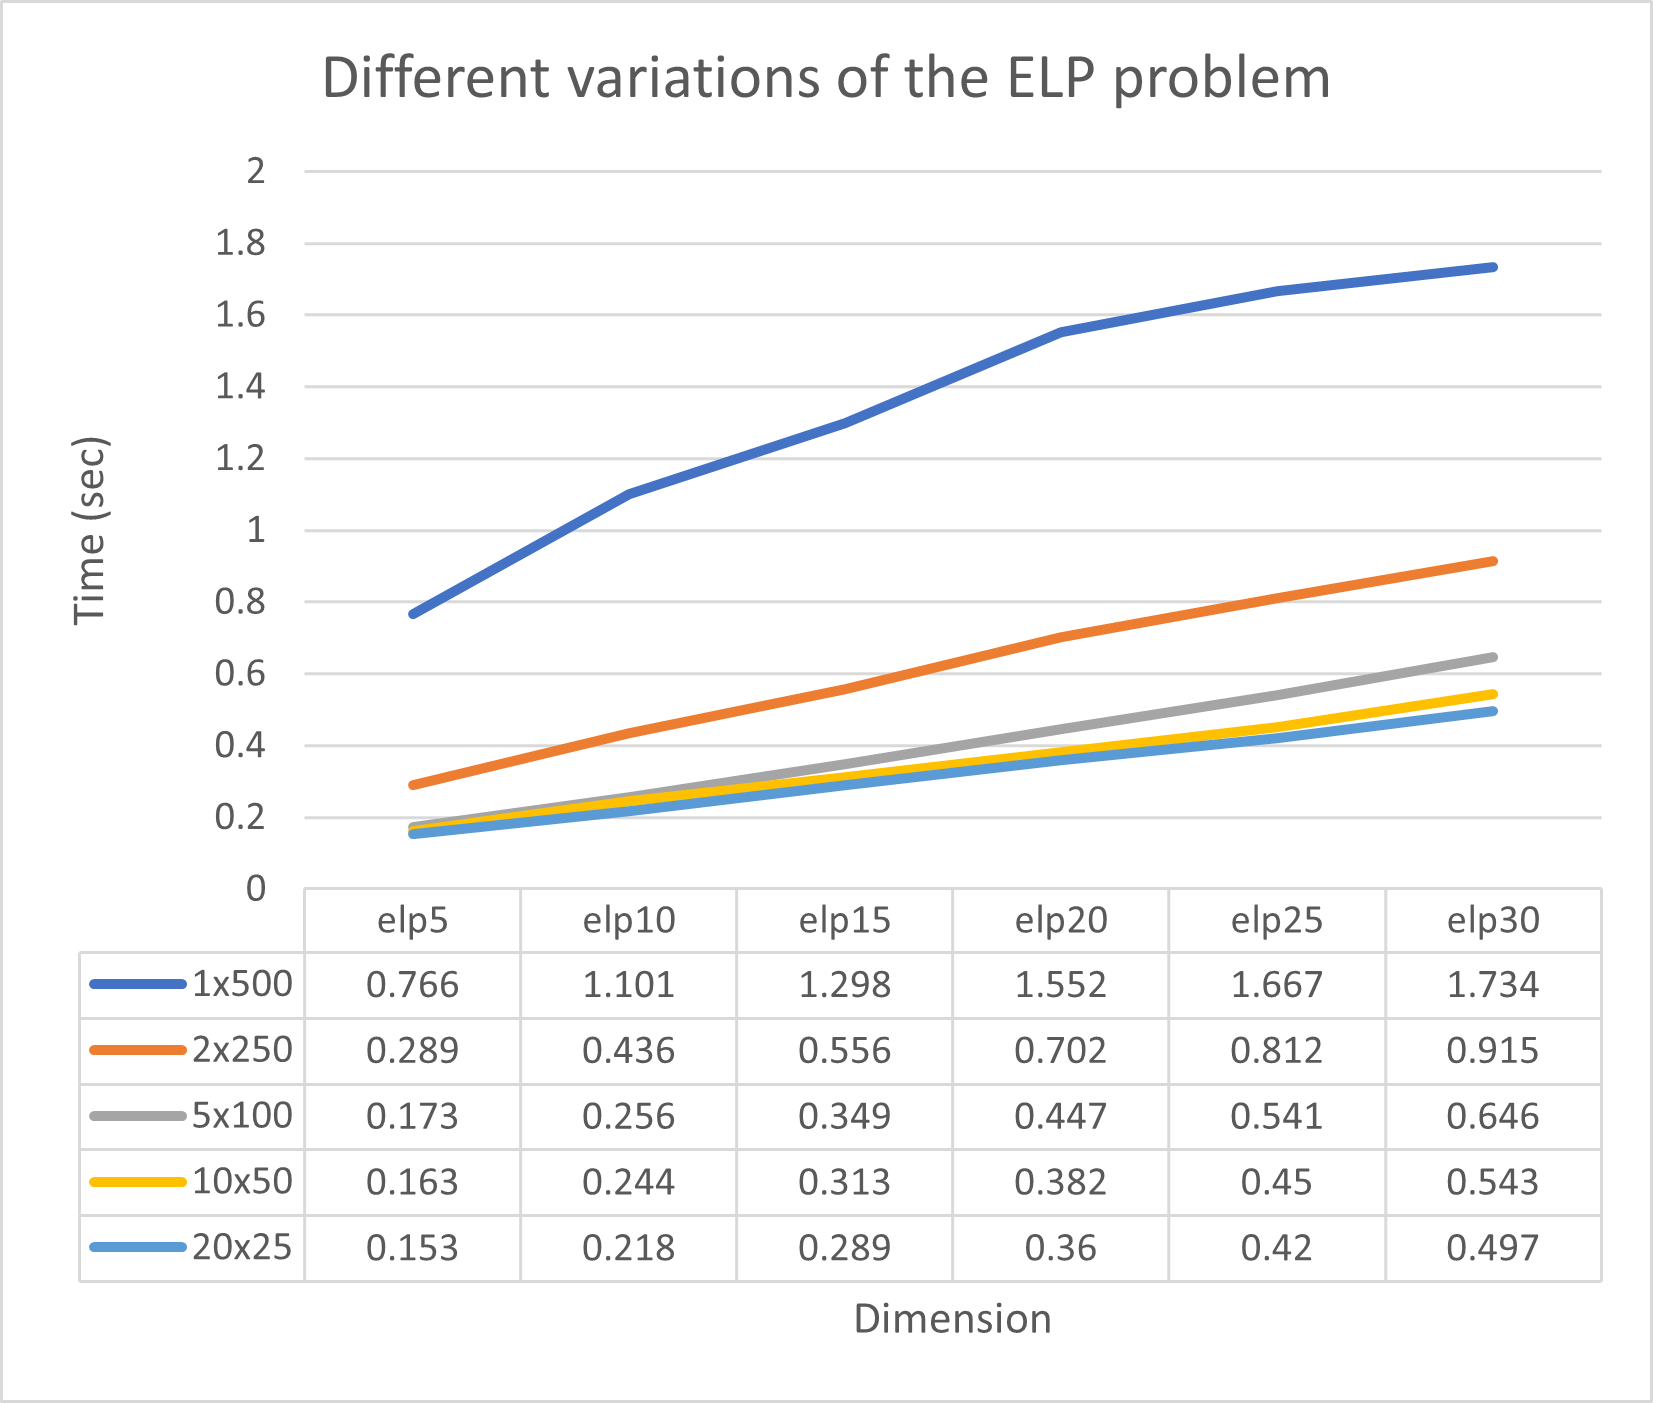
\includegraphics{11}\caption{Different variations of the ELP problem\label{fig:Comparison6}}
\par\end{centering}
\end{figure}

In Figure \ref{fig:Comparison6}, it is observed that with the collaboration
of sublisting units, the process of finding minima is significantly
accelerated.

\section{Conclusions \label{sec:Conclusions}}

According to the relevant literature, despite the high success rate
they exhibit in finding good functional values, genetic algorithms
require significant computational power, leading to longer processing
times. This manuscript introduces a parallel technique for global
optimization, where a genetic algorithm is employed to solve the problem.
Specifically, the initial population of chromosomes is divided into
various subpopulations that run on different computational units.
During the optimization process, the islands operate independently
but periodically exchange chromosomes with good functional values.
The number of chromosomes participating in migration is limited by
the crossover and mutation rates. Additionally, periodic local optimization
is performed on each computational unit, which, in turn, should not
require excessive computational power (function calls).

Experimental results revealed that even parallelization with just
two computational units significantly reduces both the number of function
calls and processing time, proving to be quite effective even with
more computational units. Furthermore, it was observed that the most
effective information exchange technique was the so-called '1toN,'
with a slight difference from the 'NtoN,' where a randomly selected
subpopulation sends information to all other subpopulations. Moreover,
the 'NtoN' technique, where all subpopulations send information to
all other subpopulations, seems to perform equally well.

Similar dissemination techniques have been applied to other stochastic
methods, such as the Differential Evolution (DE) method by Charilogis
and Tsoulos \citep{pde} and the Particle Swarm Optimization (PSO)
method by Charilogis and Tsoulos \citep{ppso}. In the case of Differential
Evolution, the proposed dissemination technique is '1to1' \ref{fig:Propagation-1to1}
and not '1toN' \ref{fig:Propagation-1toN} as suggested in this study.
However, in the case of PSO and GA, the recommended dissemination
technique is the same.

The parallelization of various methodologies of genetic algorithms
or even different stochastic techniques for global optimization can
be explored with the aim of improving the methodology. However, in
such heterogeneous environments, more efficient termination criteria
are required, or even their combined use.

\vspace{6pt}

$ $

\authorcontributions{I.G. Tsoulos conceptualized the idea and methodology, supervised
the technical aspects related to the software, and contributed to
manuscript preparation. V. Charilogis conducted the experiments using
various datasets, performed statistical analysis, and collaborated
with all authors in manuscript preparation. All authors have reviewed
and endorsed the conclusive version of the manuscript.}

\funding{This research received no external funding.}

\institutionalreview{Not applicable.}

\informedconsent{Not applicable.}

\dataavailability{Not applicable.}

\acknowledgments{This research has been financed by the European Union : Next Generation
EU through the Program Greece 2.0 National Recovery and Resilience
Plan , under the call RESEARCH -- CREATE -- INNOVATE, project name
“iCREW: Intelligent small craft simulator for advanced crew training
using Virtual Reality techniques\textquotedbl{} (project code:TAEDK-06195).}

\conflictsofinterest{The authors have no conflicts of interest to declare.}

\appendixtitles{no}

\appendixstart{}

\appendix

\begin{adjustwidth}{-\extralength}{0cm}{}


\reftitle{References}
\begin{thebibliography}{999}
\bibitem{go1}A. Törn, A. Žilinskas, Global optimization (Vol. 350,
pp. 1-255). Berlin: Springer-Verlag, 1989.

\bibitem{go_review}D. Fouskakis, D. Draper, Stochastic optimization:
a review. International Statistical Review \textbf{70}, pp. 315-349,
2002.

\bibitem{go_med1}Y. Cherruault, Global optimization in biology and
medicine, Mathematical and Computer Modelling \textbf{20}, pp. 119-132,
1994.

\bibitem{go_med2}Eva K. Lee, Large-Scale Optimization-Based Classification
Models in Medicine and Biology, Annals of Biomedical Engineering \textbf{35},
pp 1095-1109, 2007.

\bibitem{go_chem1}A. Liwo, J. Lee, D.R. Ripoll, J. Pillardy, H. A.
Scheraga, Protein structure prediction by global optimization of a
potential energy function, Biophysics \textbf{96}, pp. 5482-5485,
1999.

\bibitem{go_chem2}W.H. Shin, J.K. Kim, D.S. Kim, C. Seok, GalaxyDock2:
Protein--ligand docking using beta-complex and global optimization,
J. Comput. Chem. \textbf{34}, pp. 2647-- 2656, 2013.

\bibitem{go_physics1}Q. Duan, S. Sorooshian, V. Gupta, Effective
and efficient global optimization for conceptual rainfall-runoff models,
Water Resources Research \textbf{28}, pp. 1015-1031 , 1992.

\bibitem{go_physics2}L. Yang, D. Robin, F. Sannibale, C. Steier,
W. Wan, Global optimization of an accelerator lattice using multiobjective
genetic algorithms, Nuclear Instruments and Methods in Physics Research
Section A: Accelerators, Spectrometers, Detectors and Associated Equipment
\textbf{609}, pp. 50-57, 2009.

\bibitem{go_physics3}E. Iuliano, Global optimization of benchmark
aerodynamic cases using physics-based surrogate models, Aerospace
Science and Technology \textbf{67}, pp.273-286, 2017.

\bibitem{go_econ1}C. D. Maranas, I. P. Androulakis, C. A. Floudas,
A. J. Berger, J. M. Mulvey, Solving long-term financial planning problems
via global optimization, Journal of Economic Dynamics and Control
\textbf{21}, pp. 1405-1425, 1997.

\bibitem{go_econ2}Zwe-Lee Gaing, Particle swarm optimization to solving
the economic dispatch considering the generator constraints, IEEE
Transactions on \textbf{18} Power Systems, pp. 1187-1195, 2003.

\bibitem{go_comparison}L. Liberti, S. Kucherenko, Comparison of deterministic
and stochastic approaches to global optimization. International Transactions
in Operational Research \textbf{12}, pp. 263-285, 2005.

\bibitem{go_interval1}M.A. Wolfe, Interval methods for global optimization,
Applied Mathematics and Computation \textbf{75}, pp. 179-206, 1996.

\bibitem{go_interval2}T. Csendes and D. Ratz, Subdivision Direction
Selection in Interval Methods for Global Optimization, SIAM J. Numer.
Anal. \textbf{34}, pp. 922--938, 1997. 

\bibitem{go_determ1}C.D Maranas, C.A. Floudas, A deterministic global
optimization approach for molecular structure determination, J. Chem.
Phys. \textbf{100}, 1247, 1994.

\bibitem{go_determ2}J. Barhen, V. Protopopescu, D. Reister, TRUST:
A Deterministic Algorithm for Global Optimization, Science \textbf{276},
pp. 1094-1097, 1997.

\bibitem{go_determ3}Y. Evtushenko, M.A. Posypkin, deterministic approach
to global box-constrained optimization, Optim Lett \textbf{7}, pp.
819--829, 2013.

\bibitem{go_aco1}M. Dorigo, M. Birattari and T. Stutzle, Ant colony
optimization, IEEE Computational Intelligence Magazine \textbf{1},
pp. 28-39, 2006.

\bibitem{go_aco2}K. Socha, M. Dorigo, Ant colony optimization for
continuous domains, European Journal of Operational Research 185,
pp. 1155-1173, 2008.

\bibitem{go_crs1}W. L. Price, Global optimization by controlled random
search, Journal of Optimization Theory and Applications \textbf{40},
pp. 333-348, 1983.

\bibitem{go_crs2}Ivan Křivý, Josef Tvrdík, The controlled random
search algorithm in optimizing regression models, Computational Statistics
\& Data Analysis \textbf{20}, pp. 229-234, 1995.

\bibitem{go_crs3}M.M. Ali, A. Törn, and S. Viitanen, A Numerical
Comparison of Some Modified Controlled Random Search Algorithms, Journal
of Global Optimization \textbf{11},pp. 377--385, 1997.

\bibitem{go_pso1}J. Kennedy and R. Eberhart, \textquotedbl Particle
swarm optimization,\textquotedbl{} Proceedings of ICNN'95 - International
Conference on Neural Networks, 1995, pp. 1942-1948 vol.4, doi: 10.1109/ICNN.1995.488968.

\bibitem{go_pso2}Ioan Cristian Trelea, The particle swarm optimization
algorithm: convergence analysis and parameter selection, Information
Processing Letters \textbf{85}, pp. 317-325, 2003.

\bibitem{go_pso3}Riccardo Poli, James Kennedy kennedy, Tim Blackwell,
Particle swarm optimization An Overview, Swarm Intelligence \textbf{1},
pp 33-57, 2007. 

\bibitem{go_anneal1}S. Kirkpatrick, CD Gelatt, , MP Vecchi, Optimization
by simulated annealing, Science \textbf{220}, pp. 671-680, 1983.

\bibitem{go_anneal2}L. Ingber, Very fast simulated re-annealing,
Mathematical and Computer Modelling \textbf{12}, pp. 967-973, 1989.

\bibitem{go_anneal3}R.W. Eglese, Simulated annealing: A tool for
operational research, Simulated annealing: A tool for operational
research \textbf{46}, pp. 271-281, 1990.

\bibitem{go_de1}R. Storn, K. Price, Differential Evolution - A Simple
and Efficient Heuristic for Global Optimization over Continuous Spaces,
Journal of Global Optimization \textbf{11}, pp. 341-359, 1997.

\bibitem{go_de2}J. Liu, J. Lampinen, A Fuzzy Adaptive Differential
Evolution Algorithm. Soft Comput \textbf{9}, pp.448--462, 2005.

\bibitem{ga1}D. Goldberg, Genetic Algorithms in Search, Optimization
and Machine Learning, Addison-Wesley Publishing Company, Reading,
Massachussets, 1989.

\bibitem{ga2}Z. Michaelewicz, Genetic Algorithms + Data Structures
= Evolution Programs. Springer - Verlag, Berlin, 1996.

\bibitem{ga3}S.A. Grady, M.Y. Hussaini, M.M. Abdullah, Placement
of wind turbines using genetic algorithms, Renewable Energy \textbf{30},
pp. 259-270, 2005.

\bibitem{go_meta1}I. BoussaïD, J. Lepagnot, P. Siarry, P., A survey
on optimization metaheuristics. Information sciences \textbf{237},
pp. 82-117, 2013.

\bibitem{go_meta2}T. Dokeroglu, E. Sevinc, T. Kucukyilmaz, A. Cosar,
A survey on new generation metaheuristic algorithms. Computers \&
Industrial Engineering \textbf{137}, 106040, 2019.

\bibitem{go_meta3}K. Hussain, M.N.M. Salleh, S. Cheng, Y. Shi, Metaheuristic
research: a comprehensive survey.Artificial Intelligence Review \textbf{52},
pp. 2191-2233, 2019.

\bibitem{Holland} Holland, J.H. Genetic algorithms. Sci. Am. 1992,
267, 66--73.

\bibitem{Stender} Stender, J. Parallel Genetic Algorithms: Theory
\& Applications; IOS Press: Amsterdam, The Netherlands, 1993.

\bibitem{Goldberg} Goldberg, D. Genetic Algorithms in Search, Optimization
and Machine Learning; Addison-Wesley Publishing Company: Reading,
MA, USA, 1989.

\bibitem{Michaelewicz} Michaelewicz, Z. Genetic Algorithms + Data
Structures = Evolution Programs; Springer: Berlin/Heidelberg, Germany,
1996.

\bibitem{Santana}:Santana, Y.H.; Alonso, R.M.; Nieto, G.G.; Martens,
L.; Joseph, W.; Plets, D. Indoor genetic algorithm-based 5G network
planning using a machine learning model for path loss estimation.
Appl. Sci. 2022, 12, 3923.

\bibitem{Liu}: Liu, X.; Jiang, D.; Tao, B.; Jiang, G.; Sun, Y.; Kong,
J.; Chen, B. Genetic algorithm-based trajectory optimization for digital
twin robots. Front. Bioeng. Biotechnol. 2022, 9, 793782. {[}7{]}:

\bibitem{Nonoyama}Nonoyama, K.; Liu, Z.; Fujiwara, T.; Alam, M.M.;
Nishi, T. Energy-efficient robot configuration and motion planning
using genetic algorithm and particle swarm optimization. Energies
2022, 15, 2074.

\bibitem{Liu2} Liu, K.; Deng, B.; Shen, Q.; Yang, J.; Li, Y. Optimization
based on genetic algorithms on energy conservation potential of a
high speed SI engine fueled with butanol--gasoline blends. Energy
Rep. 2022, 8, 69--80.

\bibitem{Zhou} Zhou, G.; Zhu, Z.; Luo, S. Location optimization of
electric vehicle charging stations: Based on cost model and genetic
algorithm. Energy 2022, 247, 123437

\bibitem{Min} Min, D.; Song, Z.; Chen, H.; Wang, T.; Zhang, T. Genetic
algorithm optimized neural network based fuel cell hybrid electric
vehicle energy management strategy under start-stop condition. Appl.
Energy 2022, 306, 118036

\bibitem{Doewes}Doewes, R.I.; Nair, R.; Sharma, T. Diagnosis of COVID-19
through blood sample using ensemble genetic algorithms and machine
learning classifier. World J. Eng. 2022, 19, 175--182.

\bibitem{Choudhury} Choudhury, S.; Rana, M.; Chakraborty, A.; Majumder,
S.; Roy, S.; RoyChowdhury, A.; Datta, S. Design of patient specific
basal dental implant using Finite Element method and Artificial Neural
Network technique. J. Eng. Med. 2022, 236, 1375--1387.

\bibitem{Chen} Chen, Q.; Hu, X. Design of intelligent control system
for agricultural greenhouses based on adaptive improved genetic algorithm
for multi-energy supply system. Energy Rep. 2022, 8, 12126--12138.

\bibitem{openmpi}R.L. Graham, T.S. Woodall, J.M. Squyres, Open MPI:
A flexible high performance MPI. In Parallel Processing and Applied
Mathematics: 6th International Conference, PPAM 2005, Poznań, Poland,
September 11-14, 2005, Revised Selected Papers 6 (pp. 228-239). Springer
Berlin Heidelberg, 2006.

\bibitem{opemp}E. Ayguadé, N. Copty, A. Duran, J. Hoeflinger, Y.
Lin, F. Massaioli, G. Zhang, The design of OpenMP tasks. IEEE Transactions
on Parallel and Distributed systems \textbf{20}, pp. 404-418, 2008.

\bibitem{go_par1}E. Onbaşoğlu, L. Özdamar, Parallel simulated annealing
algorithms in global optimization. Journal of global optimization
\textbf{19}, pp. 27-50, 2001.

\bibitem{go_par2}J.F. Schutte, J.A. Reinbolt, B.J. Fregly, R.T. Haftka,
A.D. George, Parallel global optimization with the particle swarm
algorithm. International journal for numerical methods in engineering
\textbf{61}, pp. 2296-2315, 2004.

\bibitem{go_par3}Regis, R. G., \& Shoemaker, C. A. (2009). Parallel
stochastic global optimization using radial basis functions. INFORMS
Journal on Computing, 21(3), 411-426.

\bibitem{Tomohiro} Tomohiro Harada and Enrique Alba. 2020. Parallel
Genetic Algorithms: A Useful Survey. ACM Comput. Surv. 53, 4, Article
86 (August 2020), 39 pages. https://doi.org/10.1145/3400031.

\bibitem{ga_island0}L.A. Anbarasu, P. Narayanasamy, V. Sundararajan,
Multiple molecular sequence alignment by island parallel genetic algorithm.
Current Science, pp. 858-863, 2000.

\bibitem{ga_island1}U. Tosun, T. Dokeroglu, C. Cosar, A robust island
parallel genetic algorithm for the quadratic assignment problem. International
Journal of Production Research \textbf{51}, pp. 4117-4133, 2013.

\bibitem{ga_island2}A. Nandy, D. Chakraborty, M.S. Shah, Optimal
sensors/actuators placement in smart structure using island model
parallel genetic algorithm. International Journal of Computational
Methods \textbf{16}, 1840018, 2019.

\bibitem{pdoublepop}I.G. Tsoulos, A. Tzallas, D. Tsalikakis, PDoublePop:
An implementation of parallel genetic algorithm for function optimization.
Computer Physics Communications \textbf{209}, pp. 183-189, 2016.

\bibitem{Floudas} C.A. Floudas, P.M. Pardalos, C. Adjiman, W. Esposoto,
Z. G$\ddot{\mbox{u}}$m$\ddot{\mbox{u}}$s, S. Harding, J. Klepeis,
C. Meyer, C. Schweiger, Handbook of Test Problems in Local and Global
Optimization, Kluwer Academic Publishers, Dordrecht, 1999.

\bibitem{Montaz Ali} M. Montaz Ali, Charoenchai Khompatraporn, Zelda
B. Zabinsky, A Numerical Evaluation of Several Stochastic Algorithms
on Selected Continuous Global Optimization Test Problems, Journal
of Global Optimization \textbf{31}, pp 635-672, 2005.

\bibitem{Gaviano} M. Gaviano, D.E. Ksasov, D. Lera, Y.D. Sergeyev,
Software for generation of classes of test functions with known local
and global minima for global optimization, ACM Trans. Math. Softw.
\textbf{29}, pp. 469-480, 2003.

\bibitem{Lennard} J.E. Lennard-Jones, On the Determination of Molecular
Fields, Proc. R. Soc. Lond. A \textbf{ 106}, pp. 463--477, 1924.

\bibitem{Zabinsky} Z.B. Zabinsky, D.L. Graesser, M.E. Tuttle, G.I.
Kim, Global optimization of composite laminates using improving hit
and run, In: Recent advances in global optimization, pp. 343-368,
1992.

\bibitem{Yu} Yu, X., Gen, M. (2010). Introduction to Evolutionary
Algorithms. Springer London Dordrecht Heidelberg New York. ISBN 978-1-84996-128-8
e-ISBN 978-1-84996-129-5 DOI 10.1007/978-1-84996-129-5.

\bibitem{Lawrence} Lawrence D. (1991). Handbook Of Genetic Algorithms.
Publisher: Thomson Publishing Group (First Edition)

\bibitem{Kaelo}P. Kaelo, M.M. Ali, Integrated crossover rules in
real coded genetic algorithms, European Journal of Operational Research
\textbf{176}, pp. 60-76, 2007.

\bibitem{Powell}M.J.D Powell, A Tolerant Algorithm for Linearly Constrained
Optimization Calculations, Mathematical Programming \textbf{45}, pp.
547-566, 1989. 

\bibitem{Tsoulos}Tsoulos, I.G. Modifications of real code genetic
algorithm for global optimization. Appl. Math. Comput. 2008, 203,
598--607.

\bibitem{pde}Charilogis, V.; Tsoulos, I.G. A Parallel Implementation
of the Differential Evolution Method. Analytics 2023, 2, 17--30. 

\bibitem{ppso}Charilogis, V.; Tsoulos, I.G.; Tzallas, A. (2023).
An Improved Parallel Particle Swarm Optimization. SN Computer Science
(2023) 4:766

\bibitem{IPSO}Charilogis, V., Tsoulos, I. (2022). Toward an Ideal
Particle Swarm Optimizer for Multidimensional Functions. Information
2022, 13(5), 217; Doi:10.3390/info13050217.

\bibitem{IDE}Charilogis, V., Tsoulos, I., Tzallas, A., Karvounis,
E. (2022). Modifications for the Differential Evolution Algorithm.
Symmetry 2022,14(3),447; Doi: 10.3390/sym14030447 

\bibitem{S. Heiles}S. Heiles, R. L. Johnston, Global optimization
of clusters using electronic structure methods, Int. J. Quantum Chem.
\textbf{113}, pp. 2091-- 2109, 2013.

\end{thebibliography}

\end{adjustwidth}{}
\end{document}
